%\documentclass[first,firstsupp,handout,compress,notes,navigation]{ETHclass} 
%\documentclass[first,firstsupp,handout,notes]{ETHclass} 
\documentclass[first,firstsupp]{ETHclass} % handout
%\documentclass{ETHclass} 
%\documentclass[first,firstsupp,notes]{ETHclass} 
%\documentclass[first,firstsupp]{ETHclass}
% 
% Options for beamer:
%
% 9,10,11,12,13,14,17pt  Fontsizes
% 
% compress: navigation bar becomes smaller
% t       : place contents of frames on top (alternative: b,c)
% handout : handoutversion
% notes   : show notes
% notes=onlyslideswithnotes
%
%hyperref={bookmarksopen,bookmarksnumbered} : Needed for menues in
%                                             acrobat. Also need
%                                             pdftex as option or 
%                                             compile with
% pdflatex '\PassOptionsToPackage{pdftex,bookmarksopen,bookmarksnumbered}{hyperref} \input{file}'
% 
\usepackage{etex}
\usepackage{beamerseminar}
\usepackage{lmodern}
\usepackage{listings}
\usepackage{tikz}
\usepackage{verbatim}
\usepackage{wasysym}
\usepackage{bm,color}
\usepackage{subfigure}
\usetikzlibrary{arrows,shapes}
\usepackage[ruled, commentsnumbered]{algorithm2e}
\usepackage{pifont}
\usepackage{amsmath}
\usepackage{multicol}
\usepackage{soul}

\newcommand{\cmark}{\ding{51}}%
\newcommand{\xmark}{\ding{55}}

\tikzset{
    state/.style={
        rectangle,
        rounded corners,
        draw=black, very thick,
        minimum height=2em,
        inner sep=2pt,
        text centered,
    },
                                                                                     }

\usepackage{caption}
\usepackage{xcolor}
\usepackage{multicol}
\captionsetup[figure]{labelformat=empty}
\captionsetup[table]{labelformat=empty}
\newcommand{\bigO}{O}
\newcommand{\R}{\mathbb{R}}
\newcommand{\E}{\mathbb{E}}
\newcommand{\ML}{\mathbb{L}}
%\DeclareMathOperator{\st}{\textrm{s.t.}}
\DeclareMathOperator*{\nnz}{nnz}
\DeclareMathOperator*{\argmax}{arg\,max}
\newcommand{\Lagr}{\mathcal{L}}
\newcommand{\domain}{\mathcal{D}}
\newcommand{\stepsize}{\gamma}
\newcommand{\y}{\bm{y}}
\newcommand{\z}{\bm{z}}
\newcommand{\s}{\bm{s}}
\newcommand{\bv}{\bm{b}}
\newcommand{\uv}{\bm{u}}
\newcommand{\av}{\bm{v}}
\newcommand{\vv}{\bm{v}}
\newcommand{\Cv}{\bm{C}}
\newcommand{\wv}{\bm{w}}
\newcommand{\gv}{\bm{g}}
\newcommand{\Dv}{\bm{D}}
\newcommand{\alphav}{\bm{\alpha}}
\newcommand{\deltav}{\bm{\delta}}
\newcommand{\xv}{\bm{x}}
\newcommand{\Qv}{\bm{Q}}
\newcommand{\chiv}{\bm{\chi}}
\newcommand{\atoms}{\mathcal A}
\newcommand{\groups}{\mathcal G}
\newcommand{\row}{\text{row}}
\newcommand{\col}{\text{col}}
\newcommand{\lft}{\text{left}}
\newcommand{\rgt}{\text{right}}
\newcommand{\p}{\bm{p}}
\newcommand{\1}{\bm{1}}
%\setbeamertemplate{note page}[plain] 
%\setbeameroption{notes on second screen}
% 
% \usepackage[pdf]{pstricks}
% 
% %\setbeamertemplate{note page}[plain] 
% \setbeamertemplate{note page}{\ \\[.3cm]
% \textbf{\color{blue}Notes:}\\%[0.1cm]
% {\footnotesize %\tiny
% \insertnote}}
% %\setbeameroption{notes on second screen}
% 
% \usepackage{multimedia}
% 
\setbeamertemplate{navigation symbols}{} % suppresses all navigation symbols:
% \setbeamertemplate{navigation symbols}[horizontal] % Organizes the navigation symbols horizontally.
% \setbeamertemplate{navigation symbols}[vertical] % Organizes the navigation symbols vertically.
% \setbeamertemplate{navigation symbols}[only frame symbol] % Shows only the navigational symbol for navigating frames.
% 
\setparametertextfont{\scriptsize}
\setlabelfont{\scriptsize}
\setlength{\stockheight}{\paperheight}
% 
\title{Primal estimated sub-gradient solver for SVM}
\author{\small Lei Zhong}
\institute{\small Data Analytics Lab}
\date{\tiny \textbf{Apr. 21, 2015}} 
% 
\let\Tiny=\tiny
\setbeamertemplate{itemize item}{\textbullet} 
\setbeamertemplate{itemize subitem}{$\rightarrow$} % \lozenge \heartsuit \diamondsuit \bigstar \clubsuit \spadesuit \square \Box \small $\bigstar$
\setbeamertemplate{sections/subsections in toc}[ball]
\setbeamertemplate{items}[ball]
%
\newcommand{\titleslide}{{%{{\usebackgroundtemplate{\includegraphics[width=\paperwidth,height=\paperheight]{images/titleslide}}
\begin{frame}
 	% \frametitle{$ $} % 
 	\frametitle{Outline}
	\tableofcontents[currentsection, currentsubsection]
\end{frame}}}
%
\definecolor{dkgreen}{rgb}{0,0.6,0}
\definecolor{gray}{rgb}{0.5,0.5,0.5}
\definecolor{mauve}{rgb}{0.58,0,0.82}
%
\lstset{
	language=Java, %[Sharp]C, 				% c-sharp programming language
	numbers=left,					% where to put the line-numbers
	numberstyle=\tiny\color{gray},	% the style that is used for the line-numbers
	keywordstyle=\color{blue}\bfseries,	% keyword style
	keywordstyle=\color{blue},		% keyword style
	commentstyle=\color{dkgreen},	% comment style
	stringstyle=\color{mauve},		% string literal style
	stepnumber=1,					% the step between two line-numbers. If it's 1, each line 
									% will be numbered
	numbersep=5pt,					% how far the line-numbers are from the code
	tabsize=4,						% sets default tabsize to 2 spaces
	basicstyle=\small				% the size of the fonts that are used for the code	
}

\title{Adaptive Probabilities in Stochastic Optimization Algorithms}

\begin{document}

\begin{frame}[fragile]
  	\maketitle
\end{frame}
%
\institute{\it \tiny{Data Analytics Lab}}
\date{Apr. 21, 2015}
\author{\it Lei Zhong}
\title{\today \hspace{3.8cm} \arabic{page}}
%
\begin{frame}{}
\tableofcontents
\end{frame}

%\section{Introduction}

\begin{frame}{Motivation}
    \begin{itemize}
        \item Uniform probabilities are used in classical SGD/SDCA. 
        \item However, uniform probabilities would suffer from poor convergence rate for dataset with a diversified sparsity.
        \item Non-uniform sampling
        \item Adaptive sampling
    \end{itemize}
\end{frame}

\begin{frame}{Warm-up}
\begin{block}{Objective function}
    $f(\wv):= L(\wv)+\lambda r(\wv)$ where 
    $L(\wv) := \frac1n \sum_{i=1}^n \ell(\langle \xv_i, \wv \rangle, y_i)$
    and 
    $r(\wv) = \frac{\|\wv\|^2}{2}$
\end{block}
\begin{block}{Partial objective function}
    $f(\wv, i):= \ell(\langle \wv, \xv_i\rangle, y_i)+\frac {\lambda} {2} \|\wv\|^2$
\end{block}
\begin{itemize}
    \item Samples: $\xv$, Labels: $y$
    \item Probabilities: $p_i$
    \item Sub-gradient $\chiv_{i}(\wv^{t}) = \nabla f(\wv, i) = \ell'(y_{i}, \langle \wv^{t}, \xv_{i}\rangle)\xv_{i}+\lambda\wv^{t}$
    \item Sub-gradient $\gv_i = \frac{\chiv_{i}}{np_i}$, $\E\gv_i = \nabla f(\wv, i)$
\end{itemize}
\end{frame}

\begin{frame}{Non-uniform sampling}
Non-uniform sampling converges faster than uniform sampling for datasets with large variance by assigning higher probabilities to samples with larger norm.
\end{frame}

\begin{frame}{Theorem 1}
Firstly, we derive the $\bigO(\frac{\ln T}{T})$convergence rate for non-uniform sampling.

If we choose the step size as $\eta_t = \frac{1}{\lambda t}$, then after $T$ iterations with starting point $\wv^{0}=\bm{0}$, $\wv^*$ is the optimal value of $\wv$. It holds that
\[
    \E f\!\left(\frac1T\sum_{t=1}^T \wv^{t} \right)- f(\wv^*) \le \frac{1}{2\lambda T}\sum_{t=1}^T \frac{\E\|\gv_{i_t}^{t}\|^2}{t} 
    \overset{ \max_{t}\{\|\gv_{i_t}^t(\wv^t)\|\} \le G}{\le}
    \]
    \[
    \frac{1}{2\lambda T} \sum_{t=1}^T \frac{G^2}{t} \le \frac{G^2\ln T}{2\lambda T} 
\]
\end{frame}

\begin{frame}{Theorem 2}
Secondly, the convergence rate is $\bigO(1/T)$ if we take $\eta_t=\frac{2}{\lambda t+1}$ as step size. For the SGD Algorithm  with starting point $\wv^{0}=\bm{0}$, after T iterations, it holds that the weighted average of the iterates satisfies
\[
    \E f(\frac{2}{T(T+1)}\sum_{t=1}^{T}t \wv^{t}) - f(\wv^*) \le \frac{2}{\lambda(T+1)} \max_{t} \E\|\gv_{i_t}^{t}\|^2
    \le \frac{2G}{\lambda (T+1)}
\]
\end{frame}

\begin{frame}{Adaptive sampling}
Adaptivity means changing the probabilities when executing the algorithm according to the known information, typically useful for online algorithm.
In the paper, our main algorithms AdaSGD and AdaSDCA change the probabilities after one epoch.
\end{frame}

\begin{frame}{AdaSGD}
\begin{block}{Main idea}
    $\E f(\wv^{t+1}) - \E f(\wv^{t}) \le \frac{\eta_t}{2}(1+\frac{\lambda \eta_t}{2})\E\|\gv_{i_t}^{t}\|^2 - \eta_t\chiv_{i_t}\nabla L(\wv^{t}) - \frac{\lambda}{2} \wv^{t} \eta_t \chiv_{i_t}$
\end{block}
By Cauchy-Schwarz inequality, 
\[ 
    \E\|\gv_{i_t}^{t}\|^2 = \sum_{i=1}^n \frac{\|\chiv_i\|^2}{n^2p_i} = (\sum_{i=1}^n \frac{\|\chiv_i\|^2}{n^2p_i}) (\sum_{i=1}^n p_i) \ge (\sum_{i=1}^n \frac{\|\chiv_i\|}{n})^2
    \]

\begin{block}{Change $p_i$}
    $p_i = \frac{\|\chiv_i\|}{\sum_{j=1}^n \|\chiv_i\|}$, 
    $p_i = \frac{c_i}{\sum_{j=1}^n c_j}$
\end{block}
Where $c_i = \max\{l'(\langle \xv_i, \wv^t\rangle, y_i)\xv_i +\lambda \wv^t\}$.
\end{frame}

\begin{frame}{AdaSDCA}
\begin{block}{Duality gap}
    $f(\wv^{t})-D(\alphav^{t}) = \frac{1}{n} \sum_{i=1}^n(\ell(\xv_i^T\wv^{t})+\ell^*(-\alpha_i^{t})+\alpha_i^{t}\xv_i^T\wv^{t}).$
\end{block}

\begin{block}{Definition}
    $p_i = \frac{c_i}{\sum_{j=1}^n c_j}$
\end{block}
Where $c_i = \max\{l(\xv_i^T\wv^t)+l^*(-\alpha_i^t)+\alpha_i^t\xv_i^T\wv^t\}$.
\end{frame}


\begin{frame}{Online Adaptive SGD/SDCA}
Online algorithms modify the probability on the fly. By directly applying
\begin{itemize}
    \item SGD: $p_i = \max\{\epsilon, l'(\langle \xv_i, \wv^t\rangle, y_i)\xv_i+\lambda           \wv^t\}$
    \item SDCA: $p_i = \max\{\epsilon, l(\xv_i^T\wv^t)+l^*(-\alpha_i^t)+                            \alpha_i^t\xv_i^T\wv^t\}$
\end{itemize}
where $\epsilon = 10^{-8}$
\end{frame}

\begin{frame}{Comparison of complexity}
\begin{table}[htbp!]
    \centering
    \caption{One epoch computational cost of different algorithms}
    \label{table:compcost}
    \begin{tabular}{|l|l|}
        \hline
        \textsc{Algorithm} & cost of an epoch\\ 
        \hline
        AdaSGD & $(k+1)n\nnz$ \\
        AdaSDCA & $(k+1)n\nnz$ \\
        NonUnifSGD & $n\nnz$ \\
        NonUnifSDCA & $n\nnz$\\
        OnlineAdaSGD & $n\nnz$\\
        OnlineAdaSDCA & $n\nnz$\\
        AdaGrad & {\color{red}$nd$}\\
        AdaSDCA+ & $2n\nnz$ \\
        \hline
    \end{tabular}
\end{table}
$\nnz$ means the number of nonzero elements.
\end{frame}

\begin{frame}{Part A}
Non-Uniform Sampling Algorithms
\end{frame}

\begin{frame}{Problem}
\[
\min_{x\in\R^n} f(\wv)
\]
\begin{block}{Remark}
$f$ is a $\lambda$-strongly convex function.
\end{block}
\end{frame}

\begin{frame}{NonUnifSGD}
\begin{algorithm}[H]
    \label{alg:SGD}
    \caption{Non-Uniform Stochastic Gradient Discent}
    \SetKwInput{Init}{Initialize}
    \SetKwFor{Forloop}{for}{}{end}
    \SetAlgoLined
    \KwIn{$\lambda > 0$, $p_i = \frac{\|\xv_i\|}{\sum_{j=1}^n \|\xv_j\|}, \forall i\in \{1,\ldots,n\}.$
    }
    \KwData{$\{(\xv_i,y_i)\}_{i=1}^n$.}
    \Init{
        $\wv^{1}= \textbf{0}$.
    }
    \Forloop{ $t = 1,2, \dots ,T$}{
        Sample $i_t$ from $\{1,\ldots,n\}$ based on $\p$; \\
        Set stepsize $\eta_t \leftarrow \frac{1}{\lambda t}$; \\
        Set $\chiv_{i_t}^t(\wv^{t}) \leftarrow \ell'(\langle \wv^{t}, \xv_{i_t}\rangle, y_{i_t}) \xv_{i_t}+ \lambda \nabla r(\wv^t)$;\\
        Set $\gv_{i_t}^t \leftarrow \frac{\chiv_{i_t}^t(\wv^{t})}{np_{i_t}}$;\\
        Set $\wv^{t+1} \leftarrow \wv^{t}-\eta_t\gv_{i_t}^t$;
    }
    \KwOut{$\wv^{T+1}$}
\end{algorithm}
\end{frame}

\begin{frame}{Key inequality}
\begin{align*}\label{neq:fworigin}
    & \E[f(\wv^{t})]-f(\wv^*)   \le \\
    & \frac{\eta_t}{2}\E[\|\gv_{i_t}^t\|^2] +\frac{1-\lambda \eta_t}{2\eta_t} \E[\|\wv^{t}-\wv^*\|^2] - \frac{1}{2\eta_t}  \E[\|\wv^{t+1} - \wv^*\|^2]
\end{align*}
\end{frame}

\begin{frame}{Convergence Theorem}
\begin{theorem}
\label{theorem:basicSGD}
 Suppose $f$ is a $\lambda$-strongly convex function. If we choose the stepsize $\eta_t = \frac{1}{\lambda t }$, then after $T$ iterations of NonUnifSGD (Algorithm \ref{alg:SGD}) starting with $\wv^{1}=\bm{0}$, it holds that
    \[
        \E\big[ f\!\left(\frac1T\sum_{t=1}^T \wv^{t} \right) \big] - f(\wv^*) \le \frac{1}{2\lambda T}\sum_{t=1}^T \frac{\E[\|\gv_{i_t}^t\|^2]}{t}
    \]
    where $\gv_{i_t}^t=\frac{\chiv_{i_t}^t(\wv^{t})}{np_{i_t}}$ and the expectation is taken with respect to the distribution $\p$.
\end{theorem}
\end{frame}

\begin{frame}{Proof Snapshot}
\begin{figure}[H]
        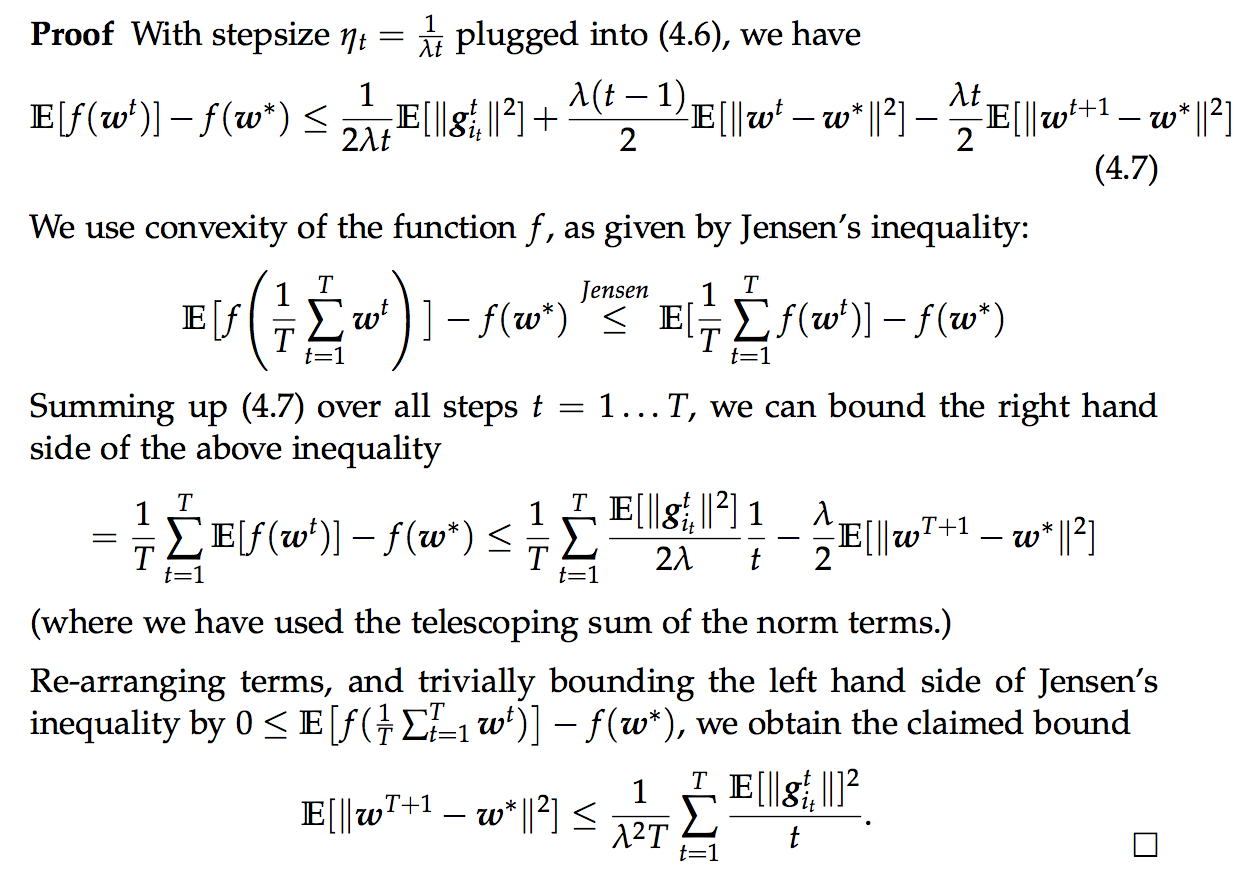
\includegraphics[width = 0.8\textwidth]{images/snapshot.png} 
    \label{fig:two_updates}
\end{figure}
\end{frame}

\begin{frame}{Two corollaries}
\begin{definition}\label{def:WG}
Define $G := \max_{i, t}\{ \|\chiv_{i}^t(\wv^{t})\|^2\}$ ($i = 1\dots n$, $t=1\dots T$).
Define $W := \max_{i,t}\{\E[\|\chiv_{i}^t(\wv^{t})\|^2]\}$ ($i = 1\dots n$, $t=1\dots T$).
\end{definition}
\begin{corollary}\label{corollary:maxsubgrad}
Assume that $\max_{t}\{\|\chiv_{i_t}^t(\wv^t)\|^2\} \le G$ for all $t$. $\E[\|\chiv_{i_t}^t(\wv^t)\|^2] \le W$ for all $t$ and $p_i > \epsilon$ for all $i=\{1\dots, n\}$,
    \begin{align*}
        \E\big[f\!\left(\frac1T\sum_{t=1}^T \wv^{t} \right)\big]- f(\wv^*) \le \frac{1}{2\lambda T} \sum_{t=1}^T \frac{G}{\epsilon nt}
\le \frac{G(\ln T+1)}{2\lambda \epsilon nT}\\
        \E\big[f\!\left(\frac1T\sum_{t=1}^T \wv^{t} \right)\big]- f(\wv^*)  \le \frac{1}{2\lambda T}\sum_{t=1}^T \frac{W}{n^2\epsilon^2 t}
\le \frac{W(\ln T+1)}{2\lambda Tn^2\epsilon^2}
    \end{align*}
\end{corollary}
\end{frame}

\begin{frame}{NonUnifSDCA}
\begin{algorithm}[H]
    \label{alg:SDCA}
    \caption{Non-Uniform Stochastic Dual Coordinate Ascent}
    \SetKwInput{Init}{Initialize}
    \SetKwFor{Forloop}{for}{}{end}
    \SetAlgoLined
    \KwIn{$\lambda > 0$, $p_i = \frac{\|\xv_i\|}{\sum_{j=1}^n \|\xv_j\|}$, $\forall i\in \{1,\ldots,n\}$.
    }
    \KwData{$\{(\xv_i,y_i)\}_{i=1}^n$}
    \Init{
        $\alphav^1 = \bm{0}$, $\wv^{1}= \bm{0}$.    }
    \Forloop{ $t = 1,2, \dots ,T$}{
        Sample $i_t$ from $\{1,\ldots,n\}$ based on $\p$; \\
        Calculate $\Delta \alpha_{i_t}^{t} = \argmax_{\Delta \alpha_{i_t}^t}[-\frac{\lambda n}{2}\|\wv^{t}+\frac{1}{\lambda n}\Delta \alpha_{i_t}^t \xv_{i_t} \|^2-\ell_{i_t}^*(-(\alpha_{i_t}^{t}+\Delta\alpha_{i_{t}}^t))]$; \\ 
        Set $\alpha_{i_{t}}^{t+1}\leftarrow \alpha_{i_{t}}^{t}+\Delta\alpha_{i_t}^{t}$;\\
        Set $\wv^{t+1}\leftarrow \wv^{t}+\frac{1}{\lambda n}\Delta\alpha_{i_t}^{t}\xv_{i_t} $;\\
    }
        \KwOut{$\wv^{T+1}$}
\end{algorithm}
\end{frame}

\section{Adaptive Sampling}
\begin{frame}{Part B}
\Large \center{\color{blue}{Adaptive Sampling Algorithms}}
\end{frame}

\begin{frame}{Idea behind SGD}
According to the SGD theorem, we can reduce the convergence rate by solving the following optimization problem:
\[
    \min \E\big[\|\gv_{i_t}^t\|^2\big].
\]
By the Cauchy-Schwarz inequality and the fact that $\sum_{i=1}^n p_i = 1$,
\[ 
    \E\big[\|\gv_{i_t}^t\|^2\big] = \sum_{i=1}^n \frac{\|\chiv_i\|^2}{n^2p_i} = (\sum_{i=1}^n \frac{\|\chiv_i\|^2}{n^2p_i}) (\sum_{i=1}^n p_i) \ge (\sum_{i=1}^n \frac{\|\chiv_i\|}{n})^2.
\]
The above inequality holds when 
\begin{equation*}\label{eq:p_optimal}
    p_i = \frac{\|\chiv_i\|}{\sum_{j=1}^n \|\chiv_i\|}.
\end{equation*}

\end{frame}

\begin{frame}{Two Updates}
\begin{algorithm}[H]
    \label{alg:AggUpdate}
    \caption{Aggressive Probability Update}
    \SetKwFor{Forloop}{for}{}{end}
    \SetAlgoLined
    \Forloop{$j = 1, \dots, n$} {
	Set $p_j \leftarrow \frac{c_j}{\sum_{k=1}^n c_k}$;
    }
    \end{algorithm}
\begin{algorithm}[H]    
    \label{alg:ConUpdate}
    \caption{Conservative Probability Update}
    \SetKwFor{Forloop}{for}{}{end}
    \SetAlgoLined
    Set $s \leftarrow \sum_{j=1,\dots, n, \1_i=\texttt{0}} c_j$; \\
    Set $c \leftarrow |S|$ where $S \leftarrow \{j | \1_i=\texttt{1}\}$; \\
    \Forloop {$j = 1, \dots, n$} {
	    $p_j>0$ $?$ {$p_j \leftarrow \frac{c_j}{s+c}$} $\colon$ {$p_j \leftarrow \frac{1}{s+c}$; } 
    } 
\end{algorithm} 
\Tiny $\1_i$ is a indicator function which returns $1$ if point $i$ is correctly classified during all the $k$ iterations, otherwise returns $0$.
\end{frame}

\begin{frame}{AdaSGD}
\begin{figure}[H]
        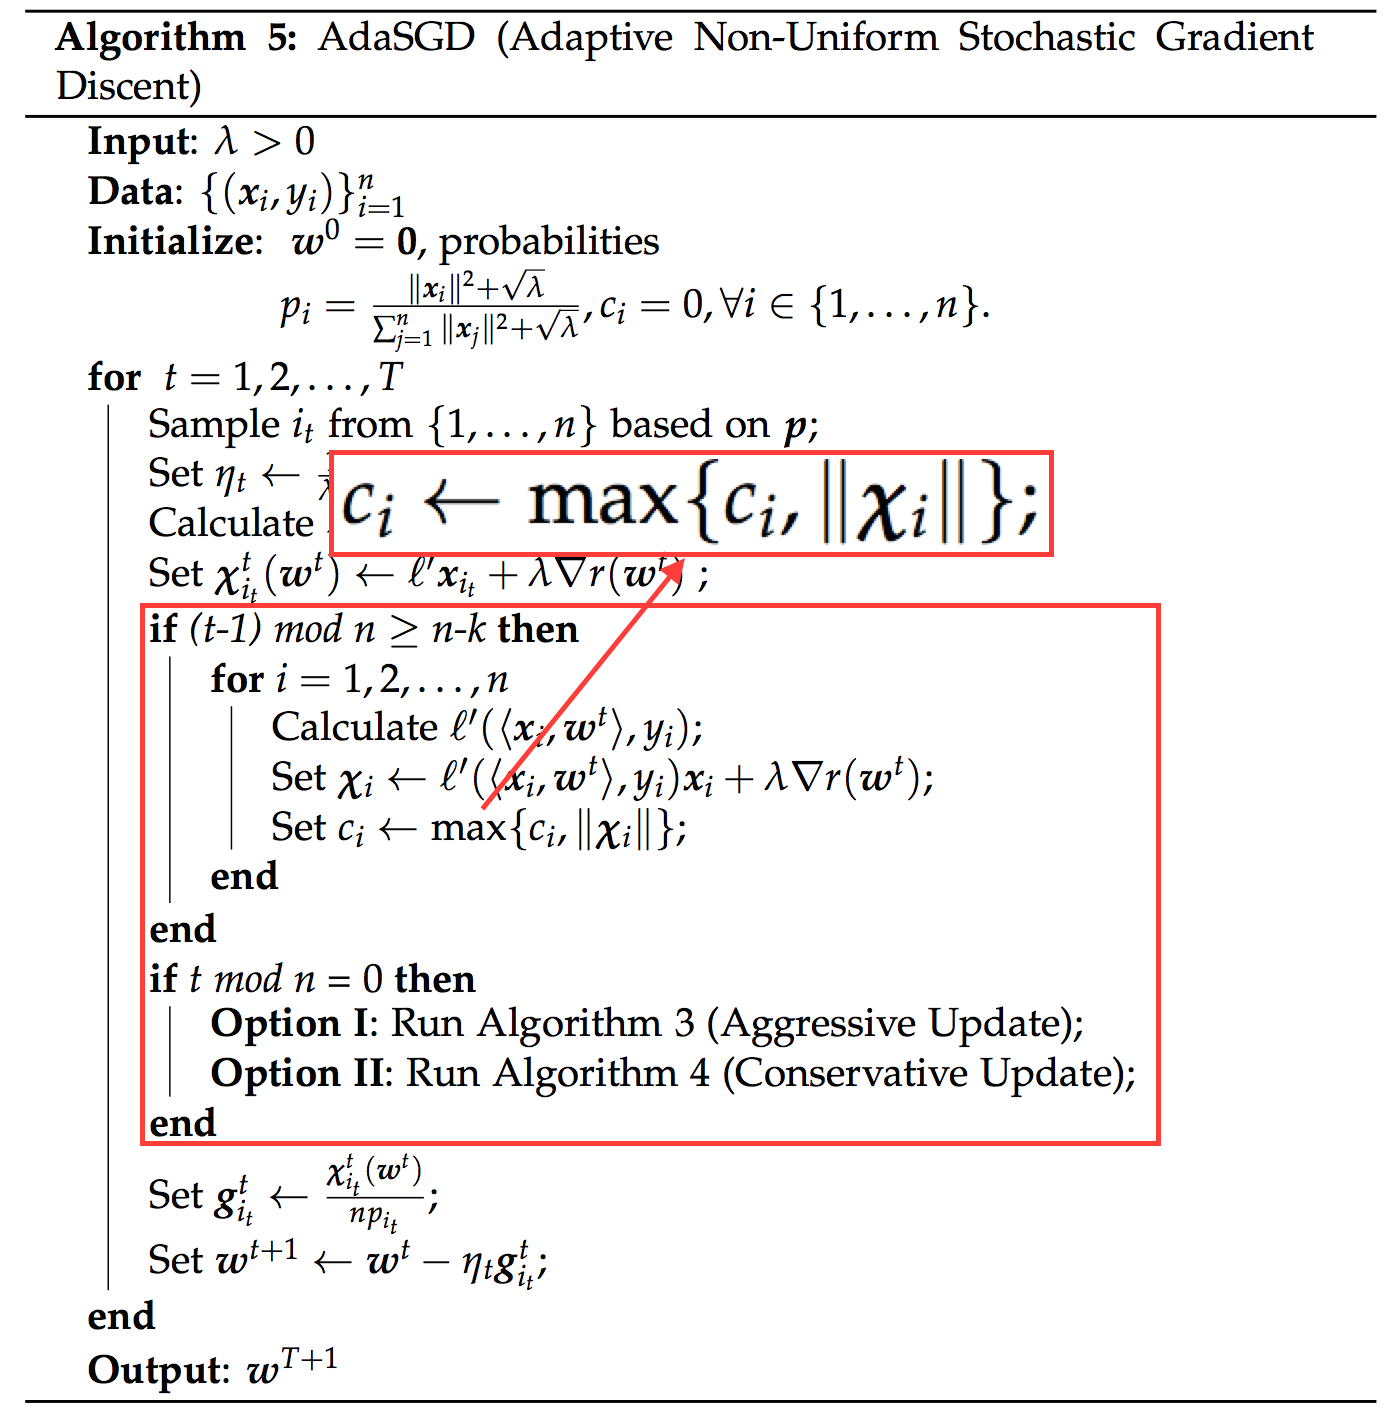
\includegraphics[height=0.8\textheight]{images/AdaSGD.png} 
    \label{fig:AdaSGD}
\end{figure}
\end{frame}

\begin{frame}{AdaSVRG}
We add a $\tilde{\wv}$ (which denotes the $\wv$ of last epoch) for a new update equation. Therefore, we get

\begin{equation*}\label{eq:vr_w_update}
    \wv^{t+1} := \wv^{t}-\eta_t [\gv_{i_t}^t(\wv^{t}) - \gv_{i_t}^t(\tilde{\wv}) - \nabla f(\tilde{\wv})]
\end{equation*}

The expectation of the update function is still the same as before, because
\[
    \E[\gv(\wv) - \gv(\tilde{\wv}) + \nabla f(\tilde{\wv})] = \E[\gv(\wv)] - \E[\gv(\tilde{\wv})] + \nabla f(\tilde{\wv}) = \nabla f(\wv).
\]
\end{frame}

\begin{frame}{Idea behind SDCA}
\begin{definition}{Define the gap of point $i$ as} 
\[
\sigma_i^t =  \ell(\xv_i^\intercal\wv^{t})+\ell^*(-\alpha_i^{t})+\alpha_i^{t}\xv_i^\intercal\wv^{t} 
\]
where $\wv^t$ here is assumed to be the corresponding primal vector for the current $\alphav^t$, that is $\wv^t(\alphav^t) := \frac{1}{\lambda n}\sum_{i=1}^n \alpha_i \xv_i^t$.
\end{definition}

The \textbf{duality gap} between the primal objective and dual objective at the $t$-th iteration is defined as
\[
    f(\wv^{t})-D(\alphav^{t}) = \frac{1}{n} \sum_{i=1}^n \sigma_i^t.
\]
\end{frame}

\begin{frame}{AdaSDCA}
\begin{figure}[H]
        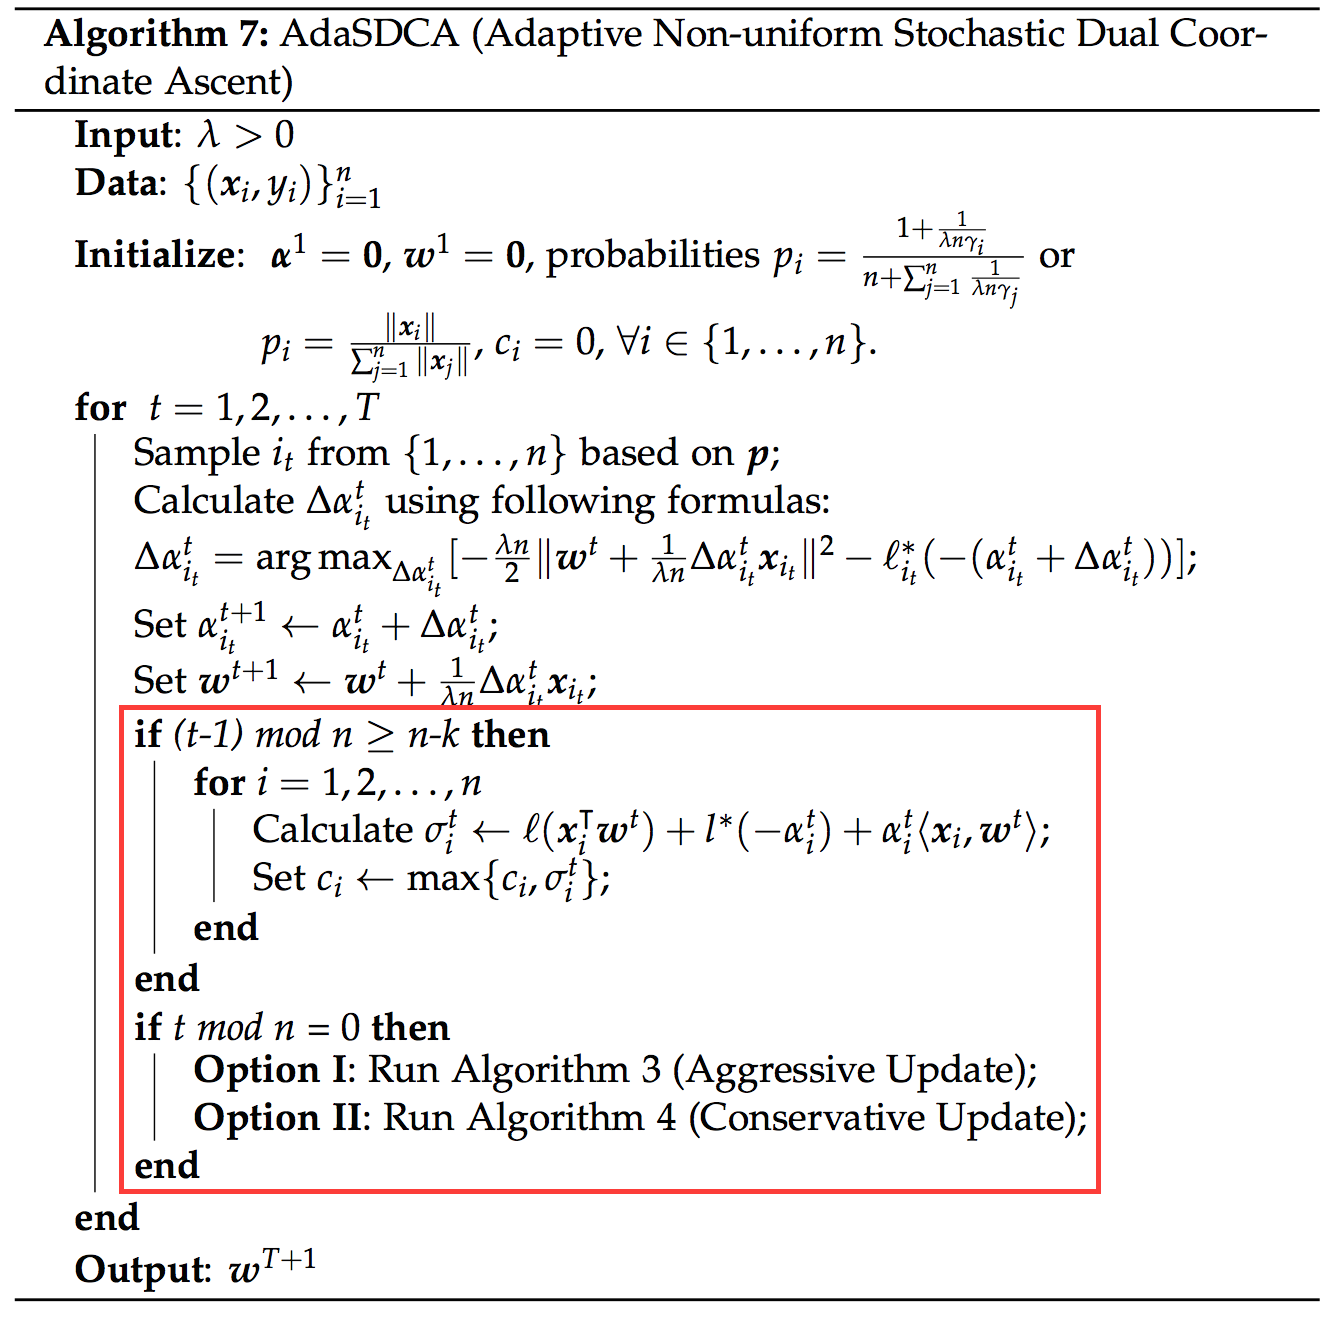
\includegraphics[height=0.8\textheight]{images/AdaSDCA.png} 
    \label{fig:AdaSDCA}
\end{figure}
\end{frame}

\begin{frame}{AdaSDCAS}
\begin{figure}[H]
        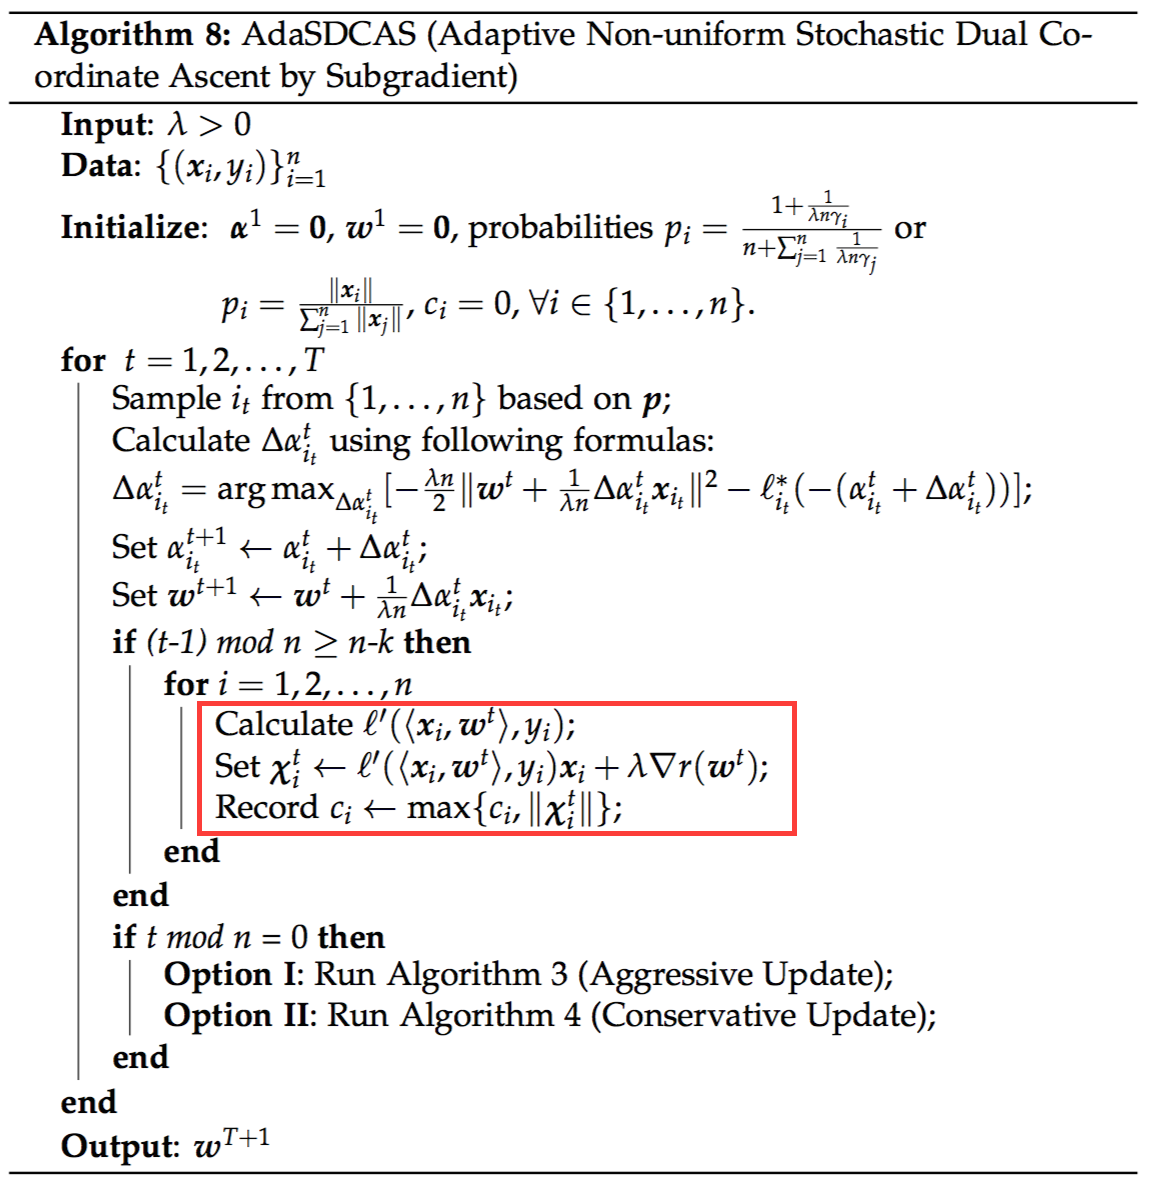
\includegraphics[height=0.8\textheight]{images/AdaSDCAS.png} 
    \label{fig:AdaSDCA}
\end{figure}
\end{frame}

%\section{Discussions and Experiments}
\begin{frame}{Part C}
\Huge \center{Discussions and Experiments}
\end{frame}

\begin{frame}{Cost per epoch and properties of algorithms}
\begin{table}[htbp]
    \centering
    \label{table:compcost}
    \begin{tabular}{|r|r|r|r|r|}
        \hline
        \textsc{Algorithm} & cost of an epoch & non-uniform & adaptive \\ 
        \hline
        NonUnifSGD & $\nnz$ & \cmark & \xmark  \\
        NonUnifSDCA & $\nnz$ & \cmark & \xmark \\
        AdaSGD & $(k+1)\nnz$ & \cmark & \cmark \\
        AdaSVRG & $nd+k\nnz$  & \cmark & \cmark \\
        AdaSDCA & $(k+1)\nnz$  & \cmark & \cmark \\
        AdaSDCAS & $(k+1)\nnz$  & \cmark & \cmark \\
        AdaGrad & $2nd$ & \xmark & \xmark \\
        Csiba-AdaSDCA & $n\nnz$  & \cmark & \cmark \\
        Csiba-AdaSDCA+ & $2\nnz$ & \cmark & \cmark \\
        \hline
    \end{tabular}
\end{table}
\end{frame}
\section{Discussions and Experiments}
\begin{frame}{Part C}
\Large \center{\color{blue}{Discussions and Experiments}}
\end{frame}

\begin{frame}{Datasets for empirical study}
\begin{table}[htbp]
    \centering
    %\caption{Datasets for empirical study} \label{table:dataset}
    \begin{tabular}{|r|r|r|r|r|r}
        \hline
        Dataset & Training($n$) & Test & Features ($d$) & Sparsity($\frac{\nnz}{nd}$) \\
        \hline
        rcv1      & 20,242 & 677,399 & 47,236 & 0.16\% \\
        \hline
        astro-ph       & 29,882  & 32,487    & 99,757 & 0.08\% \\
        \hline
    \end{tabular}
\end{table}
\begin{itemize}
\item \textbf{rcv1} is a corpus from Reuters news stories.
\item \textbf{astro-ph} is astronomy data.
\end{itemize}
\end{frame}

\begin{frame}{Cost per epoch and properties of algorithms}
\begin{table}[htbp]
    \centering
    \label{table:compcost}
    \begin{tabular}{|r|r|r|r|r|}
        \hline
        \textsc{Algorithm} & cost of an epoch & non-uniform & adaptive \\ 
        \hline
        NonUnifSGD & \textbf{nnz} & \cmark & \xmark  \\
        NonUnifSDCA & \textbf{nnz} & \cmark & \xmark \\
        AdaSGD & $(k+1)\nnz$ & \cmark & \cmark \\
        AdaSVRG & $nd+k\nnz$  & \cmark & \cmark \\
        AdaSDCA & $(k+1)\nnz$  & \cmark & \cmark \\
        AdaSDCAS & $(k+1)\nnz$  & \cmark & \cmark \\
        AdaGrad (by Duchi) & $2nd$ & \xmark & \xmark \\
        AdaSDCA (by Csiba) & $n\nnz$  & \cmark & \cmark \\
        AdaSDCA+ (by Csiba) & $2\nnz$ & \cmark & \cmark \\
        \hline
    \end{tabular}
\end{table}
\textbf{nnz}: is the number of nonzero elements of the matrix consisting of all the samples in the dataset.
\end{frame}

\begin{frame}{Test Error with Different Values of $\lambda$}
\begin{table}[htbp]
    \centering
    \begin{tabular}{|r|r|r|r|r|r|r|}
        \hline
        \texttt{rcv1} & 1e-2 & 5e-3 & \textbf{1e-3} & 5e-4 & 1e-4\\
        \hline
        Test Error & 0.05160 & 0.04833 & \textbf{0.04713} & 0.04913 & 0.05693 \\
        \hline
    \end{tabular}
\end{table}
\begin{table}[htbp]
    \begin{tabular}{|r|r|r|r|r|r|r|}
        \hline
         \texttt{astro-ph} & 1e-2 & 5e-3 & \textbf{1e-3} & 5e-4 & 1e-4 \\
        \hline
        Test Error & 0.04103 & 0.03715 & \textbf{0.03441} & 0.03586 & 0.04371 \\
        \hline
    \end{tabular}
\end{table}
\end{frame}

\begin{frame}{Verifying the Convergence of Duality Gap}
\begin{table}[htbp]
    \centering
    \caption{Average duality gap at different epochs for $\lambda = 0.001$} 
    \label{table:covdual1}
    \begin{tabular}{|r|r|r|}
        \hline
        \#epoch & duality gap on \texttt{rcv1} & duality gap on \texttt{astro-ph} \\ 
        \hline
        1 & 0.0863765 & 0.0883917\\
        3 & 0.0105347 & 6.13163e-03 \\
        10 & 1.7485e-04 & 3.93673e-05 \\
        20 & 2.21547e-05 & 6.24779e-07 \\
        50 & 3.12797e-06 & 6.7474e-10\\
        100 & \textbf{5.47897e-07} & \textbf{1.43083e-12} \\
        \hline
    \end{tabular}
\end{table}
\end{frame}

\begin{frame}{Performance Metrics}
\begin{definition}\label{def:psds}
The \textbf{primal sub-optimality} of algorithm is defined as $f(\wv) - f(\wv^*)$. 
\end{definition}
\begin{definition}
\textbf{Test error} is the error rate on test dataset.
\end{definition}
We calculate the value by 
\begin{equation*}
\ln(f(\wv)-f(\wv^*) + \epsilon).
\end{equation*}
\end{frame}

\begin{frame}{Performance of Two Updating Algorithms}
\begin{figure}[htbp]
\begin{tabular}{ll}
    \centering
        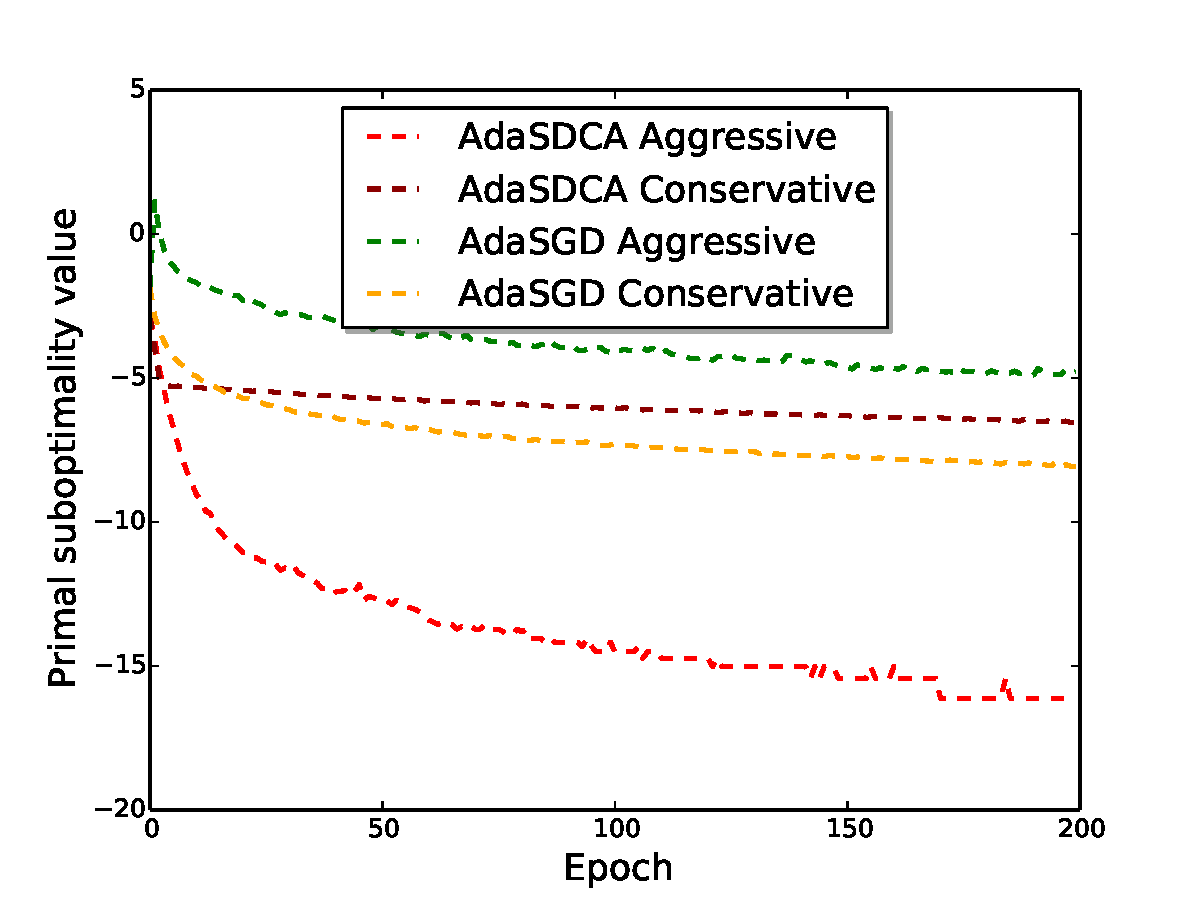
\includegraphics[width=0.5\textwidth]{images/two_updates_obej.pdf} &
        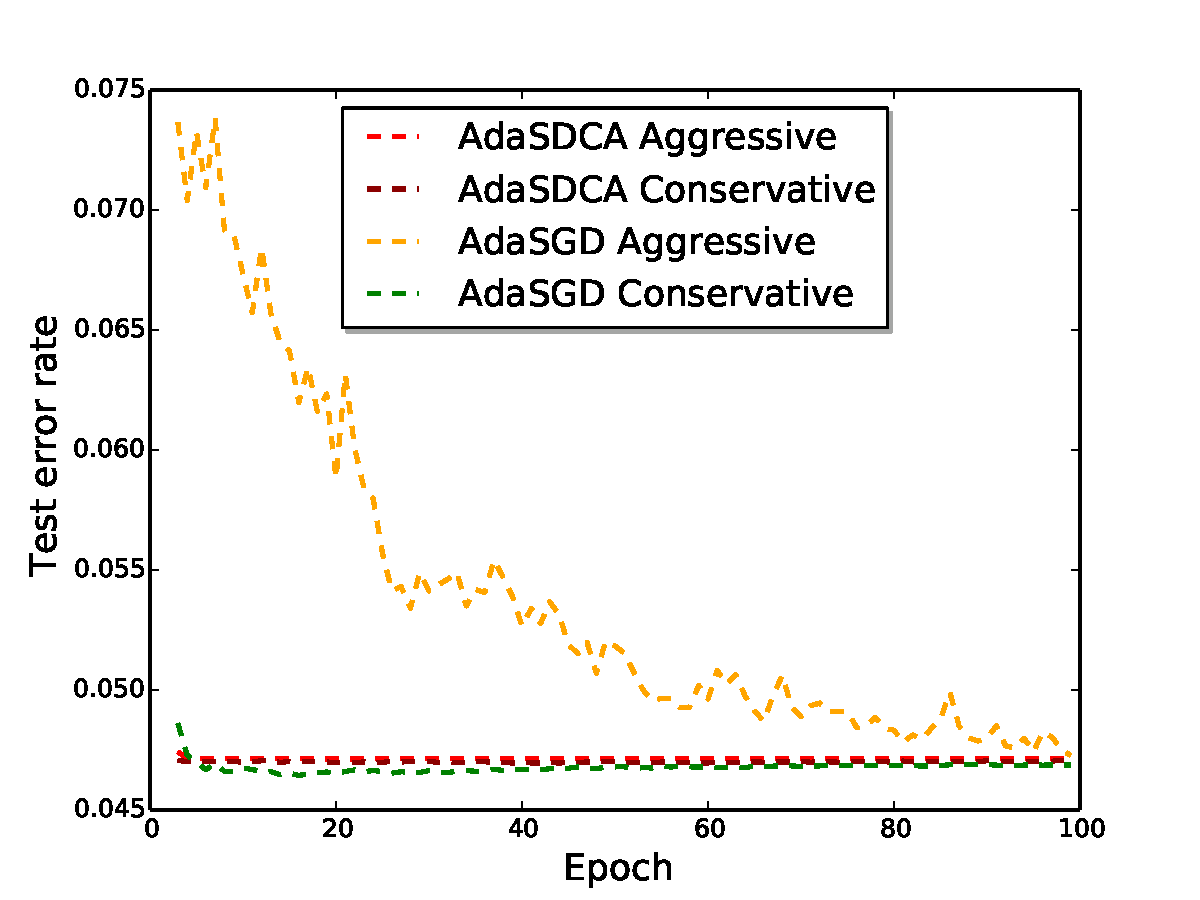
\includegraphics[width=0.5\textwidth]{images/two_updates_terror.pdf}
\end{tabular}
    \caption{Comparison of two updating algorithms for AdaSGD and AdaSDCA on \texttt{rcv1}}
    \label{fig:two_updates}
\end{figure}
\end{frame}

\begin{frame}{Different Adaptive Strategies for AdaSDCA}
\begin{figure}[htbp]
\begin{tabular}{ll}
    \centering
        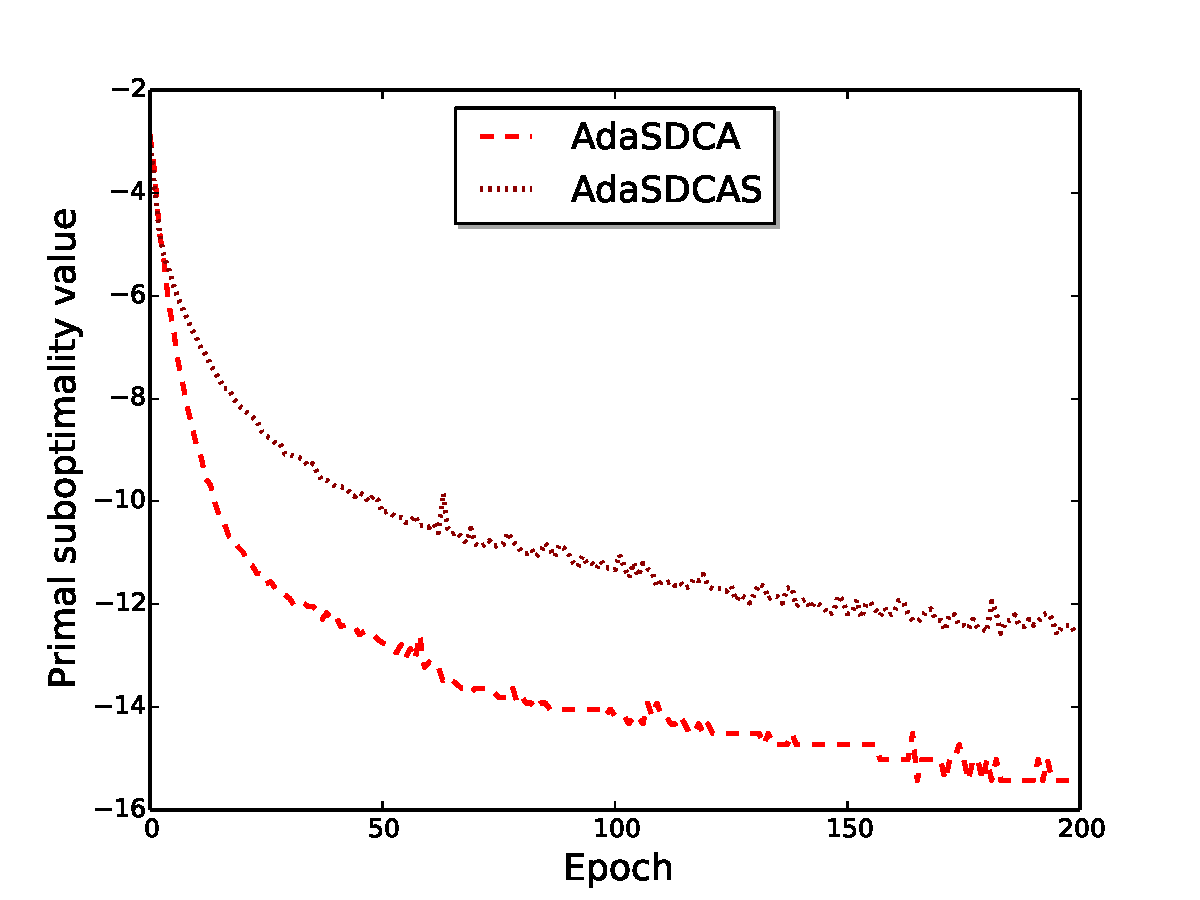
\includegraphics[width=0.5\textwidth]{images/two_strategy_SDCA_obej.pdf} &
        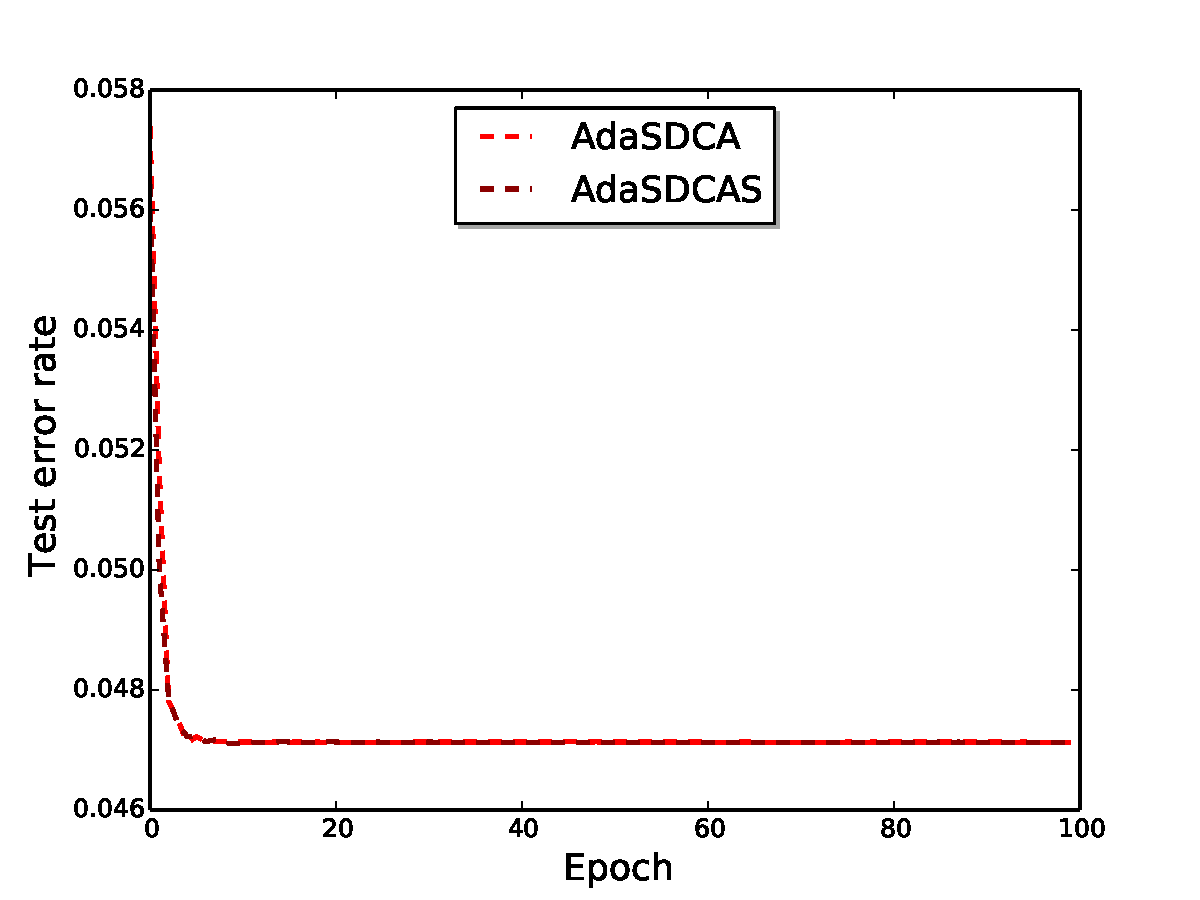
\includegraphics[width=0.5\textwidth]{images/two_strategy_SDCA_terror.pdf}
 \end{tabular}
    \caption{Comparison of AdaSDCA and AdaSDCAS on \texttt{rcv1}}
    \label{fig:sgd_on_sdca}
\end{figure}
\end{frame}

\begin{frame}{Comparison of Adaptive Algorithms}
\begin{figure}[htbp]
\begin{tabular}{ll}
    \centering
        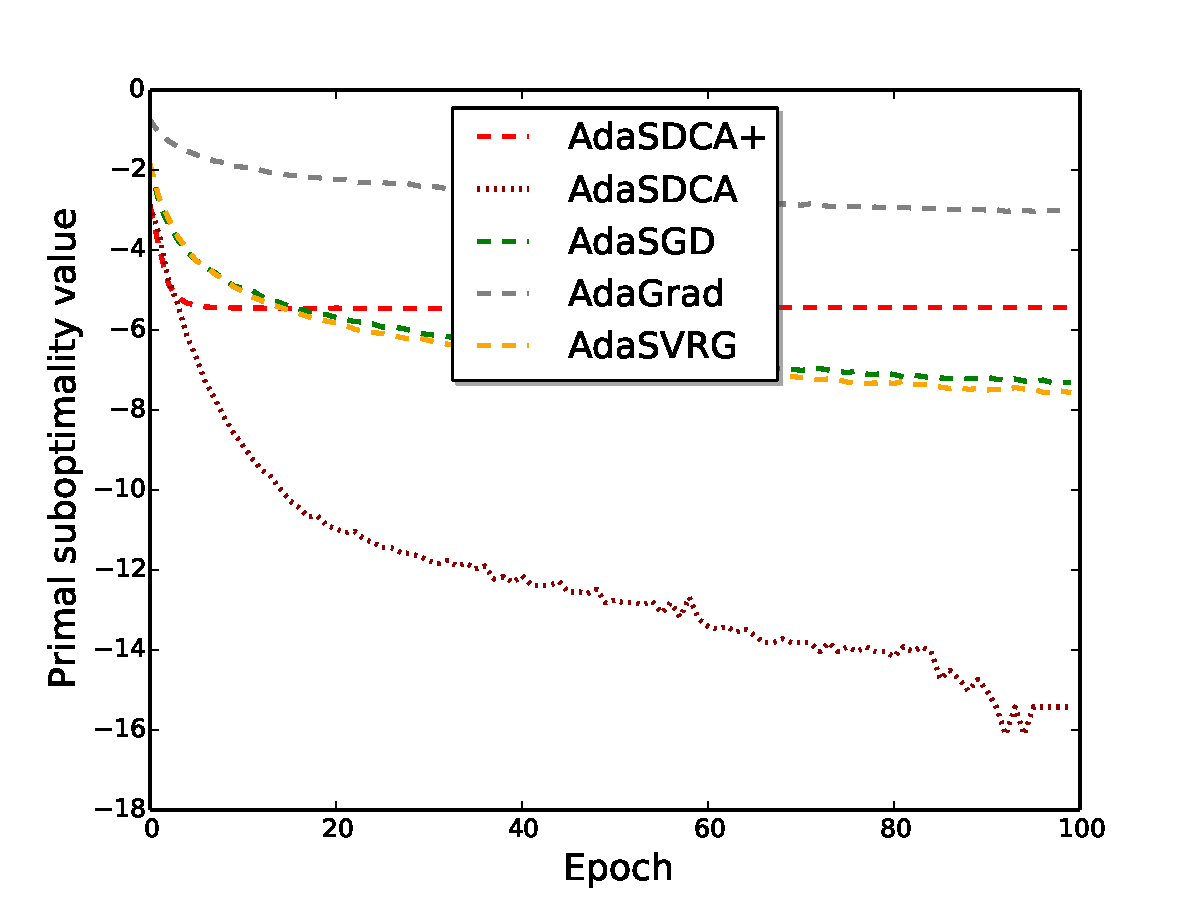
\includegraphics[width=0.5\textwidth]{images/comp_adas_obej.pdf} &
        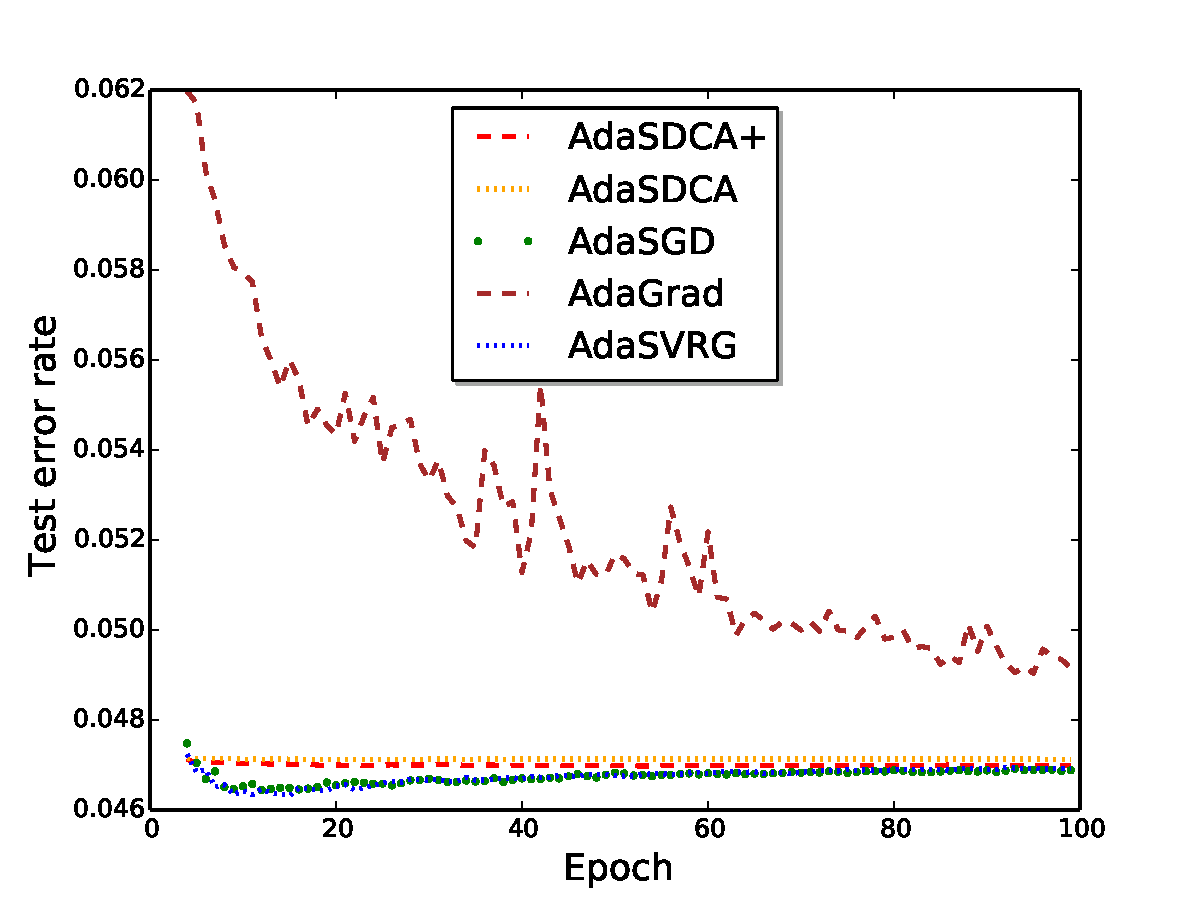
\includegraphics[width=0.5\textwidth]{images/comp_adas_terror.pdf}
        \end{tabular}
    \caption{Comparison of five adaptive algorithms on \texttt{rcv1}} 
    \label{fig:ada_all1}
\end{figure}
\end{frame}

\begin{frame}{Comparison of Adaptive Algorithms cont.}
\begin{figure}[htbp]
\begin{tabular}{ll}
    \centering
        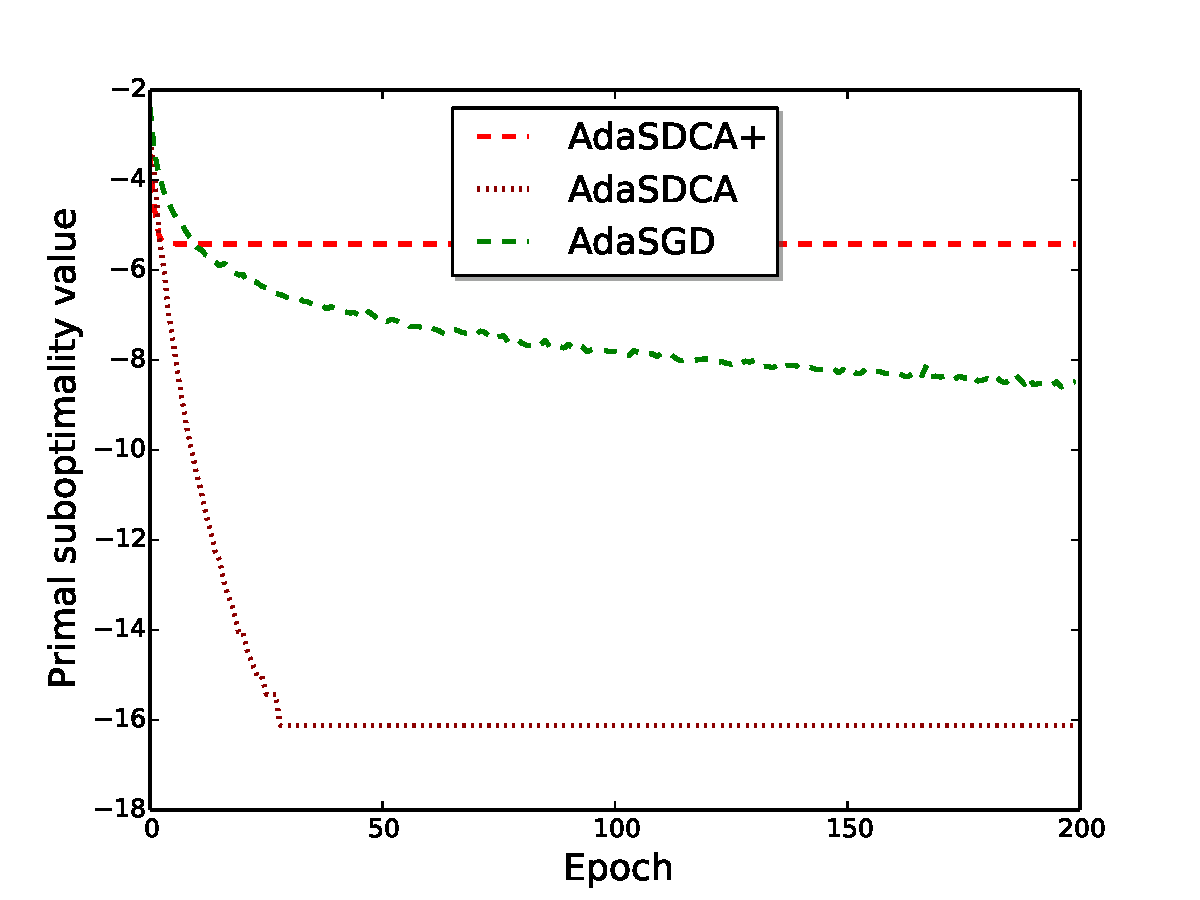
\includegraphics[width=0.5\textwidth]{images/comp_adas_obej_astro.pdf} &
        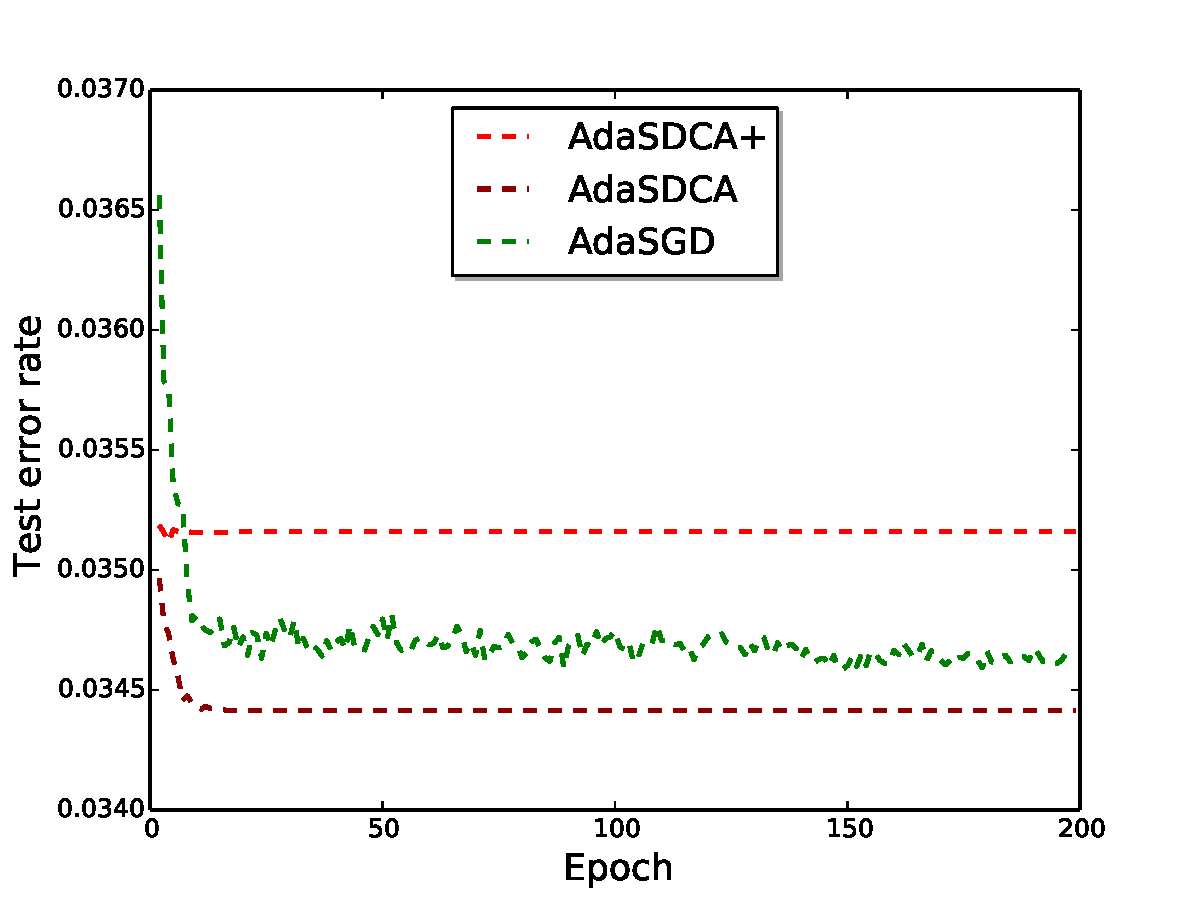
\includegraphics[width=0.5\textwidth]{images/comp_adas_terror_astro.pdf}
        \end{tabular}
    \caption{Comparison of three adaptive algorithms on \texttt{astro-ph}} 
    \label{fig:ada_all2}
\end{figure}
\end{frame}

\begin{frame}{Comparison of Average Time}
\begin{table}[htbp]
    \centering
    \caption{Detailed training time and total running time per epoch}
    \label{table:rcv1_time}
    \begin{tabular}{|r|r|r|}
        \hline 
        rcv1 & Training time(s) & Total running time(s) \\
        \hline
        AdaSGD & 0.04765 & 0.2059 \\
        \hline
        AdaSDCA & 0.05042 & 0.2064 \\
        \hline
        NonUnifSGD & \textbf{0.04244} & \textbf{0.1988} \\
        \hline
        NonUnifSDCA  & 0.04716 & 0.2037 \\
	\hline
    \end{tabular}
    \label{table:astro-ph_time}
    \begin{tabular}{|r|r|r|}
        \hline 
        astro-ph &  Training time(s) & Total running time(s) \\
        \hline
        AdaSGD & 0.07236 & 0.1363 \\
        \hline
        AdaSDCA & 0.07050 & 0.1343 \\
        \hline
        NonUnifSGD & \textbf{0.06284} & \textbf{0.1259} \\
        \hline
        NonUnifSDCA  & 0.07054 & 0.1339 \\
        \hline
    \end{tabular}
\end{table}
\end{frame}

\begin{frame}{Comparison of Time}
\begin{figure}[htbp]
\begin{tabular}{ll}
    \centering
        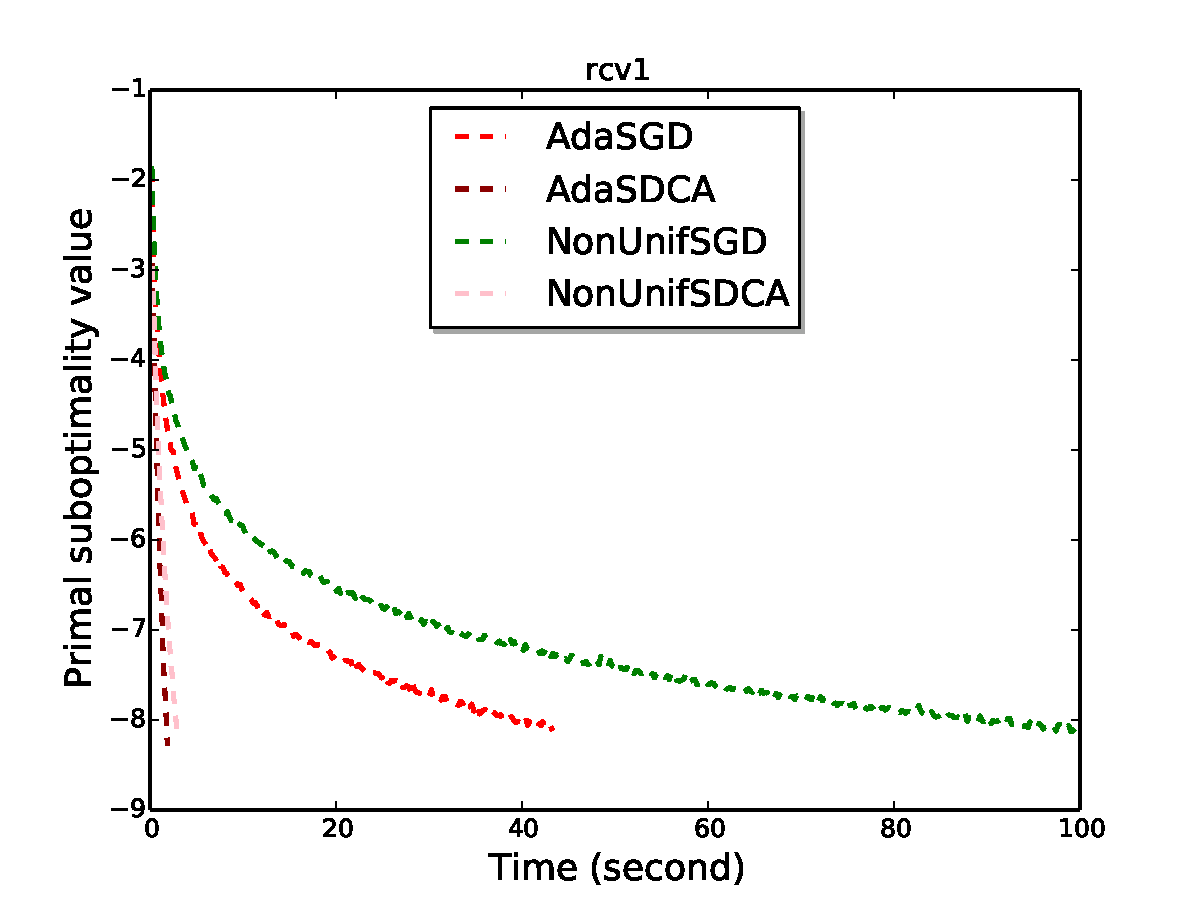
\includegraphics[width=0.5\textwidth]{images/comp_adas_time_rcv1.pdf} &
        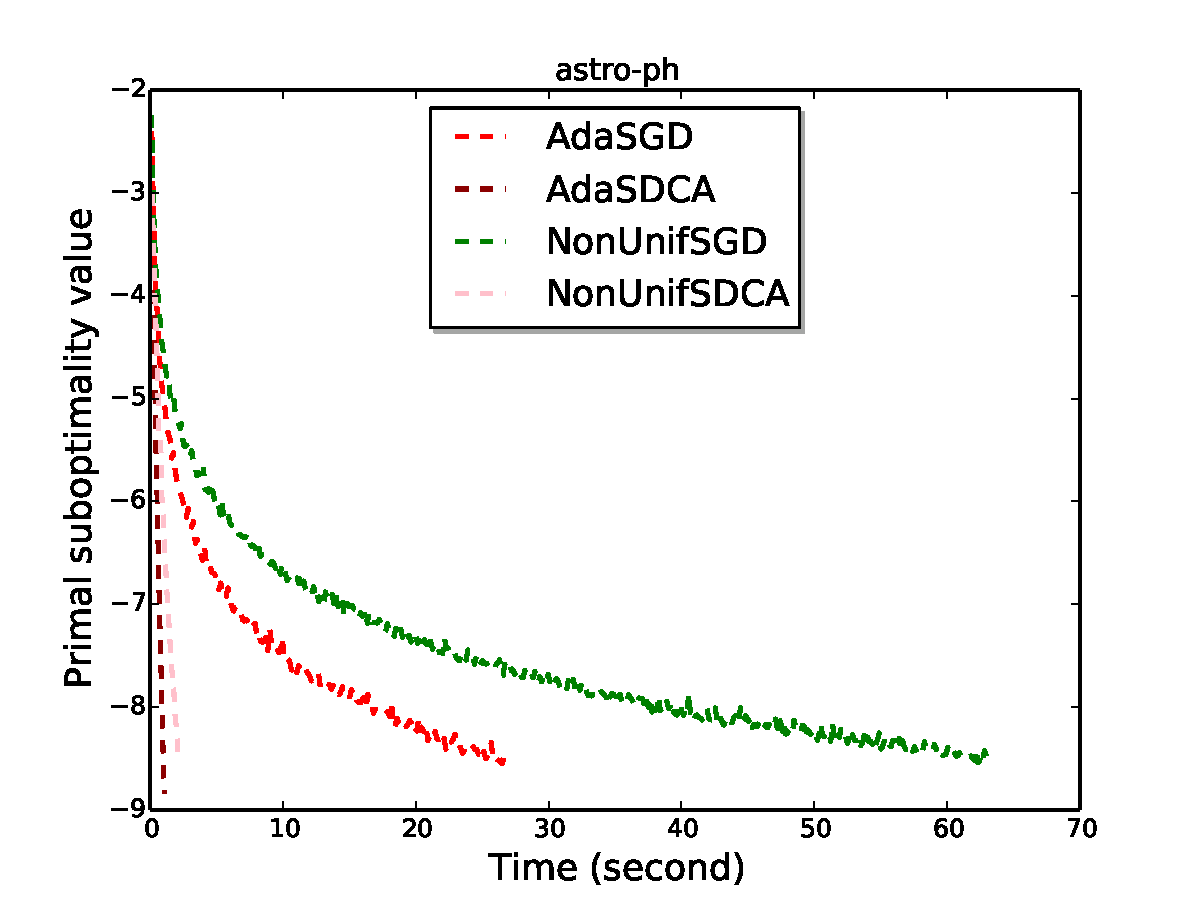
\includegraphics[width=0.5\textwidth]{images/comp_adas_time_astro.pdf}
\end{tabular}
        \caption{Comparison of the total running time to reach the same optimality}
     \label{fig:adatime}
\end{figure}
\end{frame}

\begin{frame}{Same Level of Optimality}
\begin{table}[htbp]
    \centering
    \caption{The number of epochs taken to reach the same level of optimality}
    \label{table:timetable}
    \begin{tabular}{|r|r|r|r|r|}
        \hline 
        rcv1 & AdaSDCA & NonUnifSDCA & AdaSGD & NonUnifSGD \\
        \hline
        \#epochs & \textbf{9} & 35 & 210 & 500 \\         
        \hline
    \end{tabular}
    \begin{tabular}{|r|r|r|r|r|}
        \hline 
        astro-ph & AdaSDCA & NonUnifSDCA & AdaSGD & NonUnifSGD \\
        \hline
        \#epochs & \textbf{8} & 28 & 195 & 500 \\         
        \hline
    \end{tabular}    
\end{table}
\end{frame}

\begin{frame}{Comparison of Vector Operation}
\begin{figure}[htbp]
\begin{tabular}{ll}
    \centering
        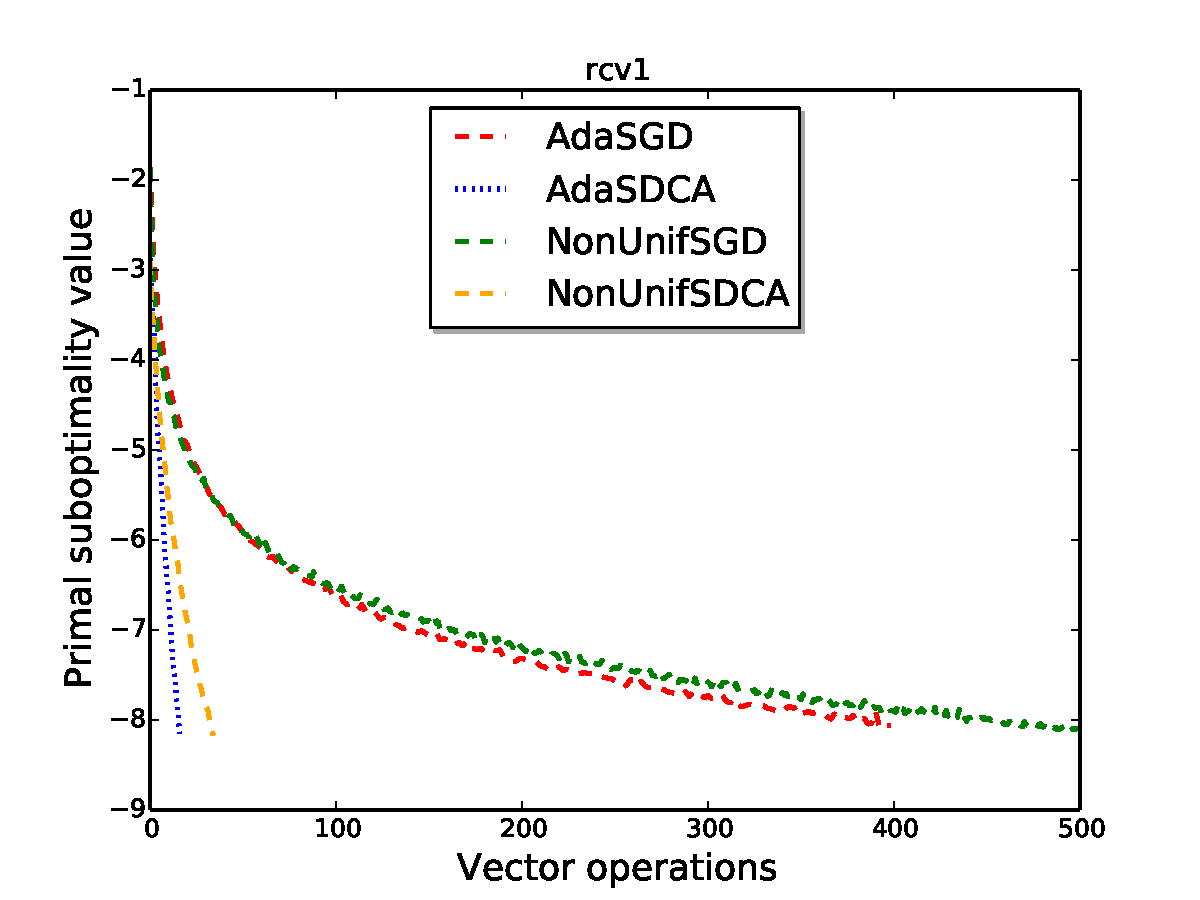
\includegraphics[width=0.5\textwidth]{images/comp_adas_vector_rcv1.pdf} &
        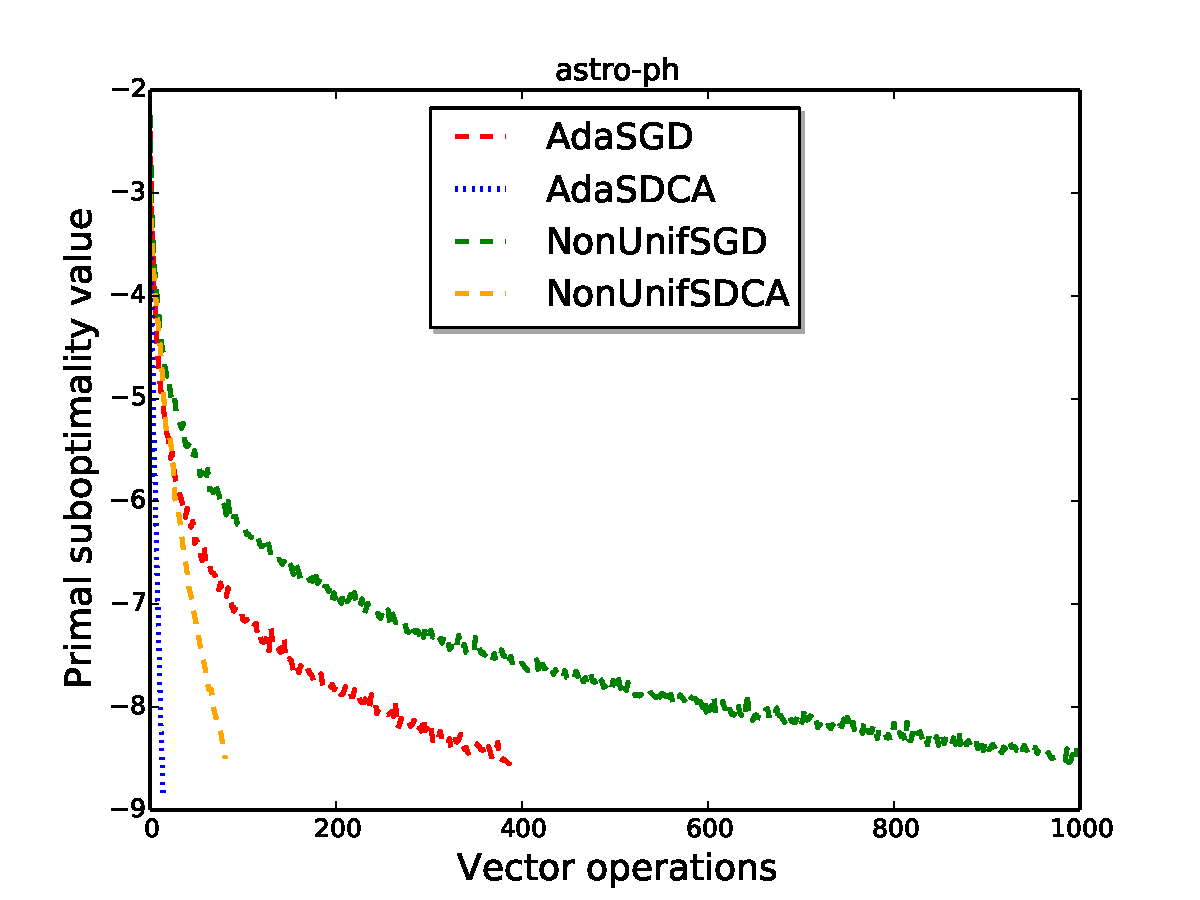
\includegraphics[width=0.5\textwidth]{images/comp_adas_vector_astro.pdf}
\end{tabular}
        \caption{Comparison of the vector operations taken to reach the same optimality}
     \label{fig:vectorop}
\end{figure}
\end{frame}

\begin{frame}{Adaptive vs. Non-Uniform Algorithms}
\begin{figure}[htbp]
\begin{tabular}{ll}
    \centering
        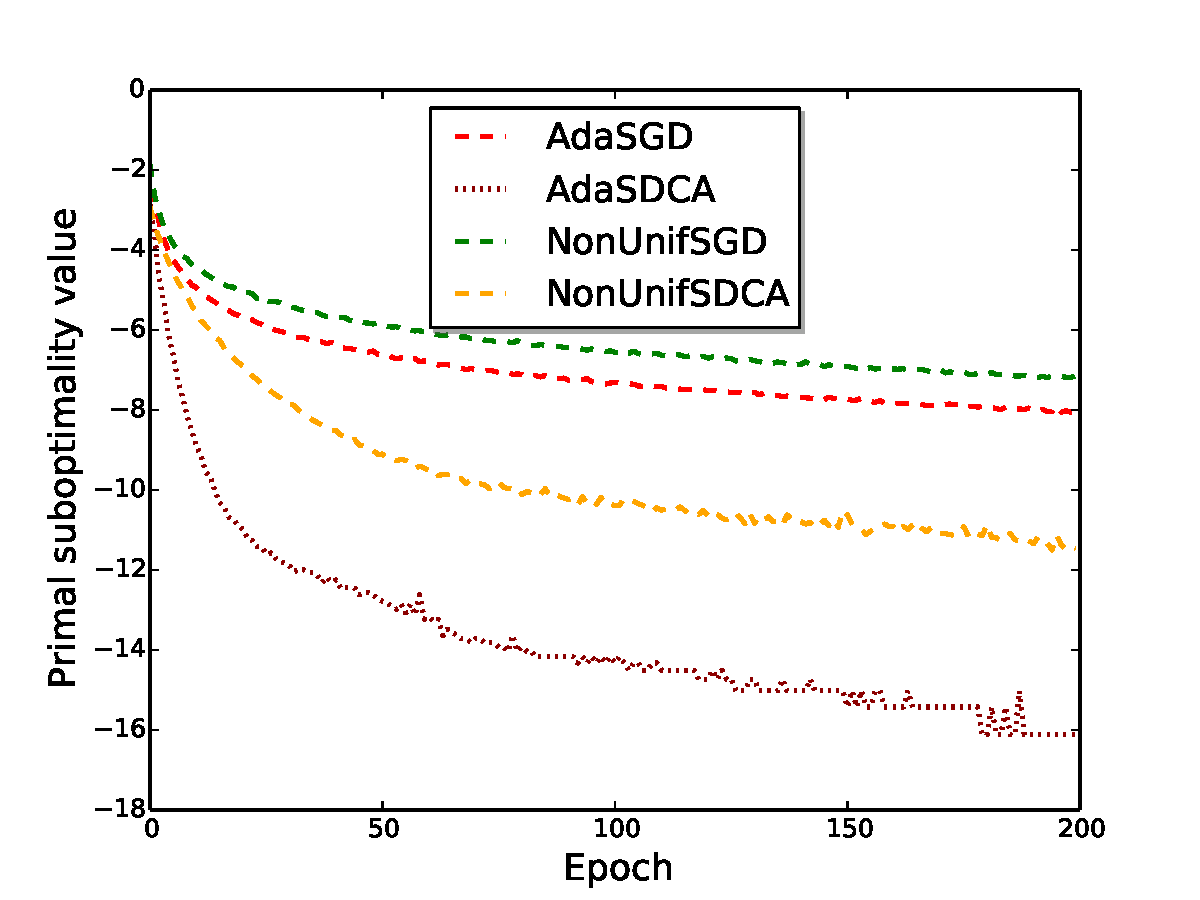
\includegraphics[width=0.5\textwidth]{images/comp_all_obej.pdf} &
        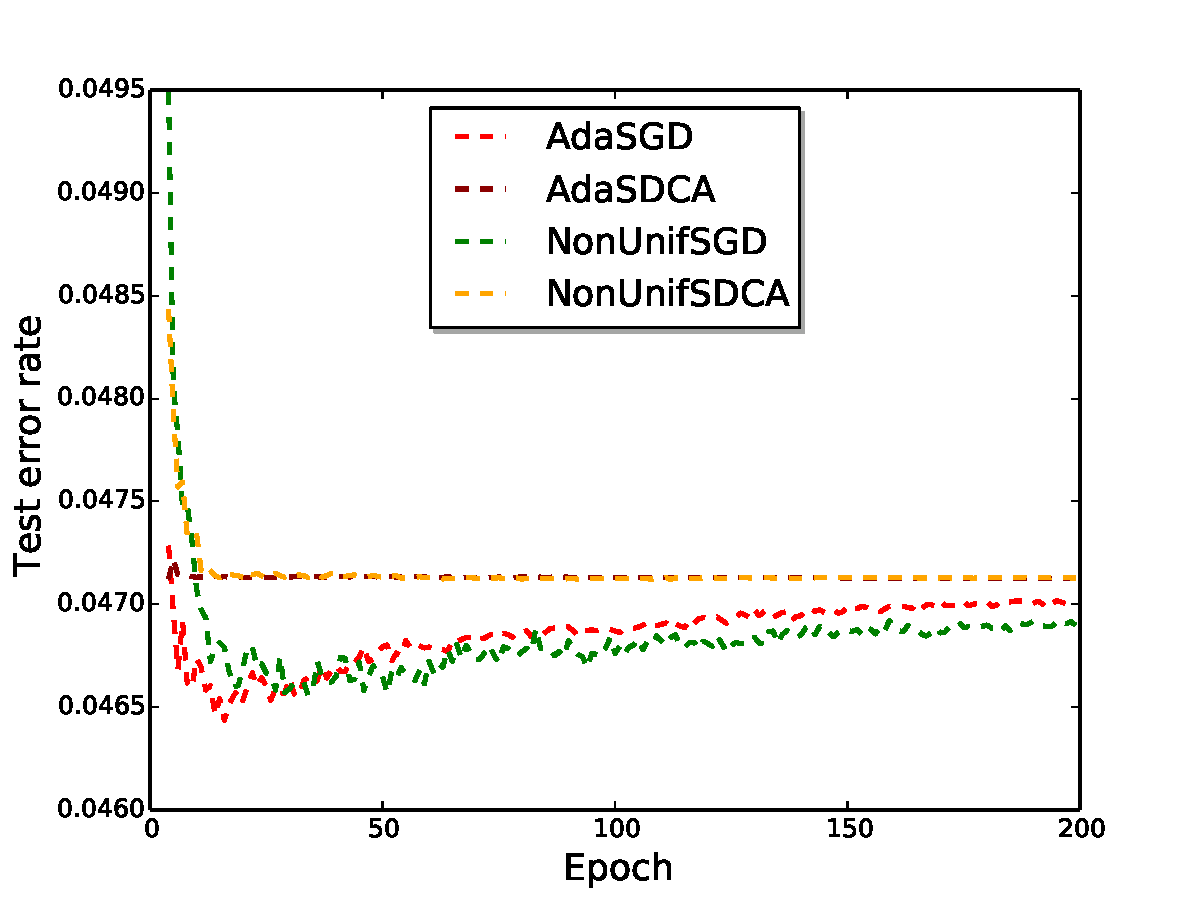
\includegraphics[width=0.5\textwidth]{images/comp_all_terror.pdf}
    \end{tabular}
    \caption{Comparison of adaptive algorithms with non-adaptive algorithms on \texttt{rcv1}} 
    \label{fig:comp_all1}
\end{figure}
\end{frame}

\begin{frame}{Adaptive vs. Non-Uniform Algorithms cont.}
\begin{figure}[htbp]
\begin{tabular}{ll}
    \centering
        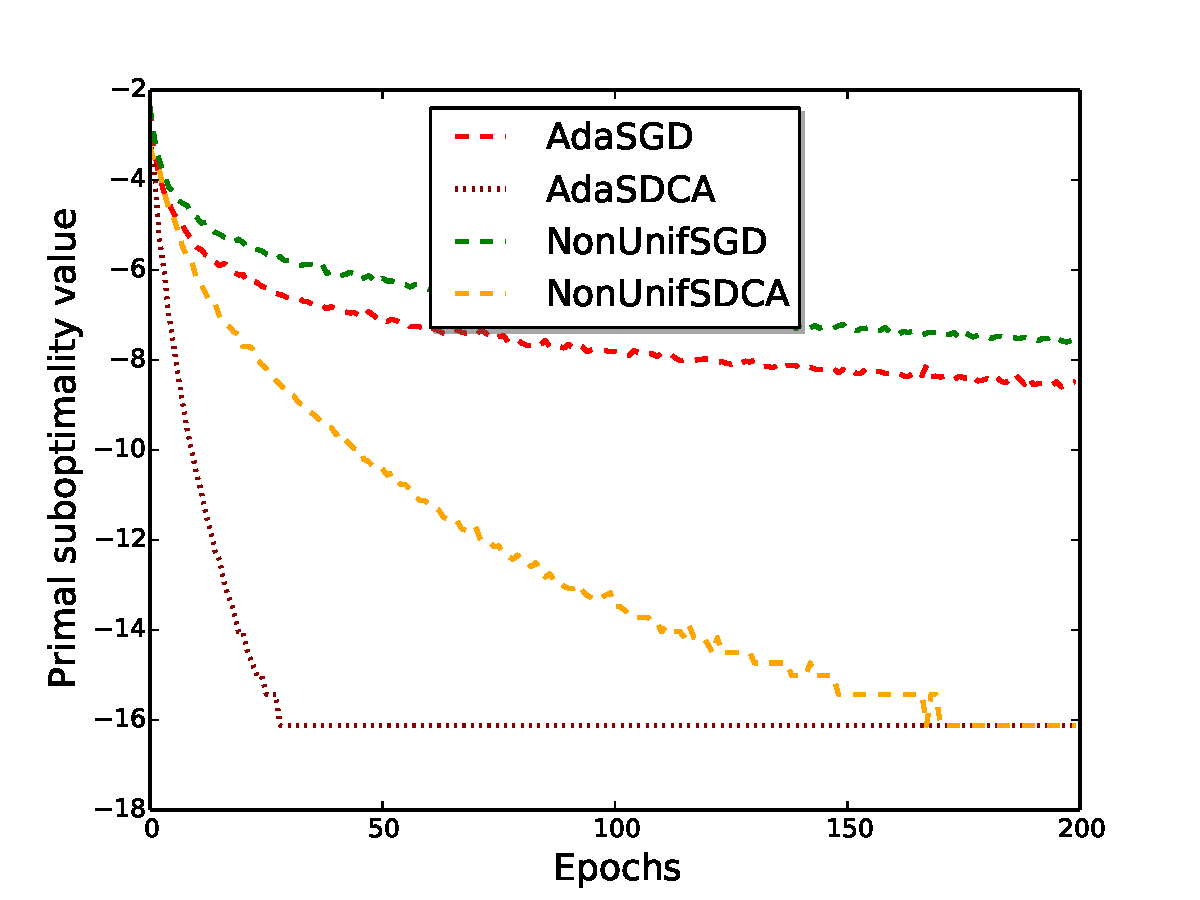
\includegraphics[width=0.5\textwidth]{images/comp_all_obej_astro.pdf} &
        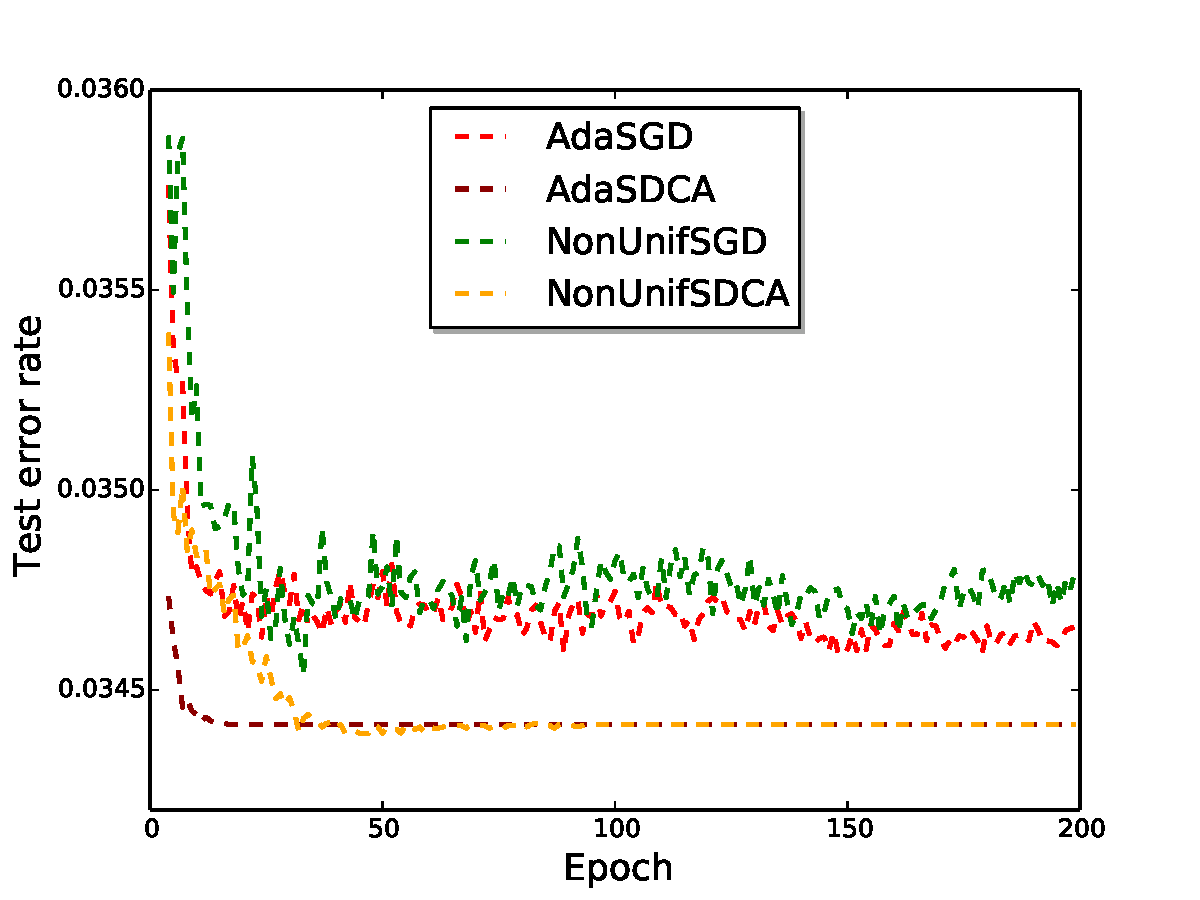
\includegraphics[width=0.5\textwidth]{images/comp_all_terror_astro.pdf}
    \end{tabular}
    \caption{Comparison of adaptive algorithms with non-adaptive algorithms on \texttt{astro-ph}} 
    \label{fig:comp_all2}
\end{figure}
\end{frame}


\begin{frame}{Summary}
\begin{itemize}
	\item Conservative Update works better on AdaSGD  while Aggressive Update works better on AdaSDCA.
	\item AdaSDCA (adaptive algorithm with duality gap) performs better than AdaSDCAS (adaptive algorithm with subgradient).
	\item AdaSDCA has the best performance among all the adaptive algorithms (AdaSDCA, AdaSGD, AdaSVRG, AdaGrad and AdaSDCA+) and AdaSGD is the second best.
	\item AdaSVRG achieves a slightly better performance per epoch than AdaSGD but sacrifices the running time on sparse datasets.
\end{itemize}
\end{frame}


\section{Reference}
\begin{frame}[fragile]
\frametitle{Reference}
\begin{itemize}
\item[] $\left[1\right]$ John Duchi, Elad Hazan, and Yoram Singer. ``Adaptive Subgradient Methods for Online Learning and Stochastic Optimization.'' JMLR, 12:21212159, August 2011.

\item[] $\left[2\right]$ Dominik Csiba, COM Zheng Qu, and Peter Richt\'arik. ``Stochastic dual coordinate ascent with adaptive probabilities.''

\item[] $\left[3\right]$ Peilin Zhao and Tong Zhang. ``Stochastic Optimization with Importance Sampling.'' arXiv.org, January 2014.

\item[] $\left[4\right]$ Zheng Qu, Peter Richt\'arik, and Tong Zhang. ``Randomized dual coordinate ascent with arbitrary sampling.'' arXiv preprint arXiv:1411.5873, 2014.

\item[] $\left[5\right]$ Rie Johnson and Tong Zhang. ``Accelerating Stochastic Gradient Descent using Pre- dictive Variance Reduction.'' In NIPS, 2013.

\end{itemize}
\end{frame}

\begin{frame}{Q\&A}
\begin{figure}[htbp]
    \begin{multicols}{2}
    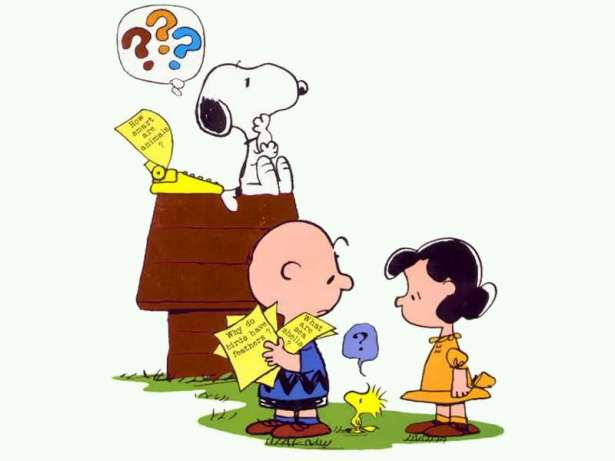
\includegraphics[height=0.4\textheight]{images/question.jpg}

    \Huge{Thank You!}
    \end{multicols}
\end{figure}

\textbf{Acknowledgement:}

Thanks to Martin for helpful discussions and suggestions!

\end{frame}



\end{document}
